\documentclass[12pt]{article}
\usepackage[utf8]{inputenc}
\usepackage{graphicx} % Allows you to insert figures
\usepackage{amsmath} % Allows you to do equations
\usepackage{fancyhdr} % Formats the header
\usepackage{geometry} % Formats the paper size, orientation, and margins
\setlength{\parindent}{0pt} % no paragraph indents
\setlength{\parskip}{1em} % paragraphs separated by one line
\usepackage[format=plain,
            font=it]{caption} % Italicizes figure captions
\usepackage[english, russian]{babel}
\usepackage{csquotes}
\renewcommand{\headrulewidth}{0pt}
\geometry{letterpaper, portrait, margin=1in}
\setlength{\headheight}{14.49998pt}
\usepackage{mathtools}
\usepackage[normalem]{ulem}
\usepackage{caption}
\usepackage{subcaption}
\usepackage{cite}
\usepackage{nicefrac}
\usepackage{wrapfig}
\usepackage{hyperref}
\usepackage{amsmath}
\usepackage{amssymb}
\usepackage{dsfont}
\usepackage[backend=bibtex, language=auto, autolang=other, bibencoding=utf8]{biblatex}
\usepackage[T1,T2A]{fontenc}% Russian language support
\addbibresource{./citation.bib}
\usepackage{algpseudocodex}

\newcommand\dout{
   \bgroup
   \markoverwith{%
       \rule[0.2ex]{0.1pt}{0.4pt}%
       \hskip-0.1pt
       \rule[0.8ex]{0.1pt}{0.4pt}%
   }
   \ULon
}
\MakeRobust\dout

\usepackage{minted}
\setminted{fontsize=\small, baselinestretch=0.8}
%\setminted[cuda]{fontsize=\small, frame=lines, framesep=2mm, baselinestretch=1.2, bgcolor=LightGray, linenos}


\newcommand\titleofdoc{GPGPU Programming with CUDA}
\newcommand\GroupName{Leo Kruglikov} 

\begin{document}
\begin{titlepage}
   \begin{center}
        \vspace*{4cm} 

        \Huge{\titleofdoc{}} 

        \vspace{0.5cm}
        \LARGE{Introduction for dummies from dummy}
            
        \vspace{3 cm}
        \Large{\GroupName}
       
       
        \vspace{3 cm}
        \Large{Personal notes}
        
        \vspace{0.25 cm}
        \Large{2022}

       \vfill
    \end{center}
\end{titlepage}

\setcounter{page}{2}
\pagestyle{fancy}
\fancyhf{}
\rhead{\thepage}


\renewcommand{\baselinestretch}{0.5}\normalsize
\tableofcontents
\renewcommand{\baselinestretch}{1}\normalsize


\section*{Author's preword}
\label{disclaimer}
These \textit{notes} are a kind of a collection of different articles from diverse resources on this topic. More precisely, the authors interpretation 
of these. A big part of the code snippets 
are also taken from different resources, 
and has not always been tested. The author will do its best to try to cite the sources. 
Therefore it is really a \textit{collage} of notes, articles, books on the CUDA programming.
The author's main goal is to provide the most detailed possible explanation of 
various code snippets, as well as try to explain the main features of CUDA programming.

Note that this document was initially written for the author itself, who is a physics major 
and is a fully self-taught guy in programming. 
For the author, it was a way of learning the topic and memorize 
the important concepts of it. 

The goal of these notes is to \textbf{give us a good basic understanding of the 
GPU architecture, and \underline{the most importantly,}, try to fully depict
the most common examples of CUDA codes}.

\section*{Dictionary}
\label{section:dictionary}
\begin{itemize}
   \setlength\itemsep{-0.5em}
   \item GPU - Graphics Processing Unit
   \item CUDA - Compute Unified Device Architecture. The language we use to \textit{talk to the GPU}. I will often refer to it as the CUDA API. In fact,
     it is not a language, but an API.
   \item Device - the GPU, from the software viewpoint. You may think of the notion of the 
   device as an external executor of a function, in our case, the GPU.
   \item Host - the CPU, from the software viewpoint. The \textit{machine}, that will launch GPU code from a
    usual \verb|C/C++| (or any other language) program, which, by default, would have been executed on the CPU.
   \item Kernel - nothing more than a function, that will run on the device(GPU).
   \item SIMT/SIMD - Single Instruction Multiple Threads/Data.
\end{itemize}



\newpage

\section*{Small introduction}
If one wants to perform computations on the GPU, one must have a way to adress it. There are various
API's developed. The biggest ones are the Khronos Group's OpenCL, Microsoft's Direct Compute, and the one 
discussed here, the Nvidia's Compute Unified Device Architecture, or shortly - CUDA. Do not mix it up with 
OpenGL, which is a slightly different thing, as it operates more on the graphics functionality.


When discussing the necessity of the GPU for computations, many come up with the example of the car and the bus \cite{habr_car_vs_bus}. 
Suppose you need to transport people from a point $A$ to a point $B$. To solve this problem, you are 
given a car and a bus. What would be the most optimized way to transport these people? We introduce here
the notion of throughput (bandwidth) and latency. The ability to perform a certain number of operations in a certain period of 
time is the throughput, and the amount of time that is required to perform a single operation is the latency.
In our analogy, the bus, having a smaller speed than the car, but a greater capacity, has a big latency but 
a big throughput. On the other hand, the car has a small latency and small throughput.


So going back to our problem, we have that if the number of people to transport is significant, 
then the wise way to transport them is to use the bus. However, if the number of people is small enough, 
one should use the car, to get the small group of people faster to the point $B$. 
In this analogy, the car is the CPU, and the bus is the GPU.

I am convinced that after some examples of code using CUDA, the reader will understand, how powerful
actually the GPGPU model is for certain tasks acomplishment. Like in our example with the bus and the car.


\newpage

\section{Basics of Architecture}

Before starting to consider some \verb|C/C++| CUDA code examples, we will look into some architecture of the GPU. 
Indeed, one of the differences between CUDA (or GPU) and usual/sequential programming (in our understanding, the
\textit{usual} programming is the code we write in C, Java, Python, etc...), 
is that one must take into account
the architecture of the GPU, while writing even some simple code. The GPU has a multithread architecture by default, 
so when the programmer is partitioning the parallel tasks, he must make sure that there is no any redundant
operations, and think about the way the cores will execute these tasks. If this partitioning takes into consideration all necessary aspects of the architecture and memory, it is possible to archive significant performance improvments.


The main difference between the CPU and the GPU is that the GPU has, in a way, lots of smaller CPU's in it, which 
are much less powerful than the actual CPU (\autoref{cpuvsgpu}).
\cite{tuomanen2018hands}

\begin{figure}
   \centering
   \includegraphics[scale=0.4]{pngs/cpuvsgpu.png}
   \caption{Schematic difference in architecture between the CPU and the GPU. Without going into details 
   (\sout{as mentionned in the disclaimer, the author have not studied it in depth}), one are able to see that 
   the GPU has many smaller ALU's. They are less powerful than those of the CPU and don't stand a chance in 
    a theoretical \textit{1v1 battle}, but may do enough \textit{damage}, when working together.\cite{tuomanen2018hands}}
   \label{cpuvsgpu}
\end{figure}

\subsection{Execution abstraction}
As you might have noticed, the GPU is by definition a multi-threaded device. This means, it is suitable for the so called 
Single Instruction Multiple Threads or SIMT (remember the bus and car analogy).


From the hardware viewpoint, we are distinguishing the \textbf{Device (GPU)} itself, the \textbf{Streaming Multiprocessors (SM's)}
, and the \textbf{CUDA cores}. These are physical entities, having a certains structure and caracteristics. 
The goal is not to give a detailed description of the GPU architecture, but rather to provide the 
idea of the CUDA mapping between the hardware and software world. While launching a kernel on the device, 
every mentionned part will be assigned a certain role, and will treat the software abstractions accordingly.

For us, the programmers, we will consider the abstraction that maps the hardware side to the software side of the program. 

\vspace{-15pt}
\paragraph{\underline{Threads}} are fundamental units of any GPU program. It is the most primitive \textit{executor} of a function 
launched on the GPU. Threads (from the software side) are executed on the \textbf{CUDA cores} (the hardware side of the program).

\vspace{-15pt}
\paragraph{\underline{Blocks}} \label{blocks} are grouping entities that enclose threads. When a function is asked to run on the GPU, the 
blocks are delegated to the corresponding \textbf{Streaming Multiprocessor} or \textbf{SM}.
So by now, we get that 

\begin{quote}
   \centering
   Block of threads $\xrightarrow[]{\text{are transmitted to}}$ SM \newline
   Threads in the block $\xrightarrow[]{\text{are executed on}}$ Cores 
\end{quote} 

So we get that the SM's are partitioning the execution of threads on the Cores at runtime. For example, suppose we have 
launched 8 blocks of lets say 32 threads each. Suppose our GPU has 2 SM's. Then, as mentionned above, 
the blocks are divided and delegated to SM's. Thus for a GPU with 2 SM's, each SM will contain 
$\nicefrac{8\text{blocks}}{2\text{SM's}} = 4 \text{blocks}$, but if our GPU has 4 SM's, 
each SM will contain $\nicefrac{8\text{blocks}}{4\text{threads}} = 2 \text{blocks}$.

\vspace{-15pt}
\paragraph{\underline{Grid}} is the top-level abstraction layer from the software's perspective. The grid
is the grouping entity that encapsulates blocks. We are thus considering that we are launching 
the grid on the \textbf{device}.
\begin{quote}
   \centering
    (Device$\xrightarrow[]{contains}$)Grid $\xrightarrow[]{\text{contains}}$ Blocks $\xrightarrow[]{\text{constains}}$ Threads
\end{quote}

\vspace{-18pt}
\paragraph{The mapping abstraction} So to recap the mentionned notions, consider the 
sketch of the hardware/software mapping.

\begin{wrapfigure}{l}{0.6\textwidth}
   %\begin{center}
      \vspace{-10pt}
      \centering
       \includegraphics[height=6cm]{pngs/hard_soft.png}
    %\end{center}
   \caption{Hardware-software abstraction}
   \label{abstraction}
\end{wrapfigure}
The abstraction between the hardware and the software side of CUDA is shown \autoref{abstraction}. Once the function 
is provided, the programmer should think of the execution pipeline through threads, blocks, and the grid.

\clearpage
\newpage
\subsection{Parallel execution and warps}
\label{warps}
We briefly saw the anatomy and the terminology of some underlying elements of the CUDA kernel execution.
Conceptually, the threads, to whom a kernel was assigned execute in parallel and are grouped into thread blocks.
Thread blocks run concurrently with each other grouped into a grid. It is important to note (see \autoref{blocks}) that 
the SM's will \textit{automatically} assign the block's execution based on the GPU resources. One may say that 
\textsl{
there is no promise on the block's concurrent execution.
}. So we do not know the order in which the blocks will be run.


However, there is a notion, which more or less guarantees the order of the execution of threads. 
The Streaming Multiprocessor
treats threads in groups of 32, which are called \underline{warps}. Think of the warps as a way to handle 
the threads, rather than 
a way of grouping (as the blocks of threads) \footnote{In the AMD terminology, a warp is reffered to as the 
\underline{wavefront}. It brings more insight into the nature of warps}.

\subsection{Memory model}
The memory model of the GPU is quite complicated. It has different fields of memory that have different characteristics-
latency of access, write/read modes, size, scope (to whom it is visible), etc... First let's take a look into 
notions concerning the memory model.
\vspace{-15pt}
\paragraph{Coalesced vs uncoalesced memory access.} 

\begin{wrapfigure}{l}{0.6\textwidth}
   %\begin{center}
      \vspace{-10pt}
      \centering
      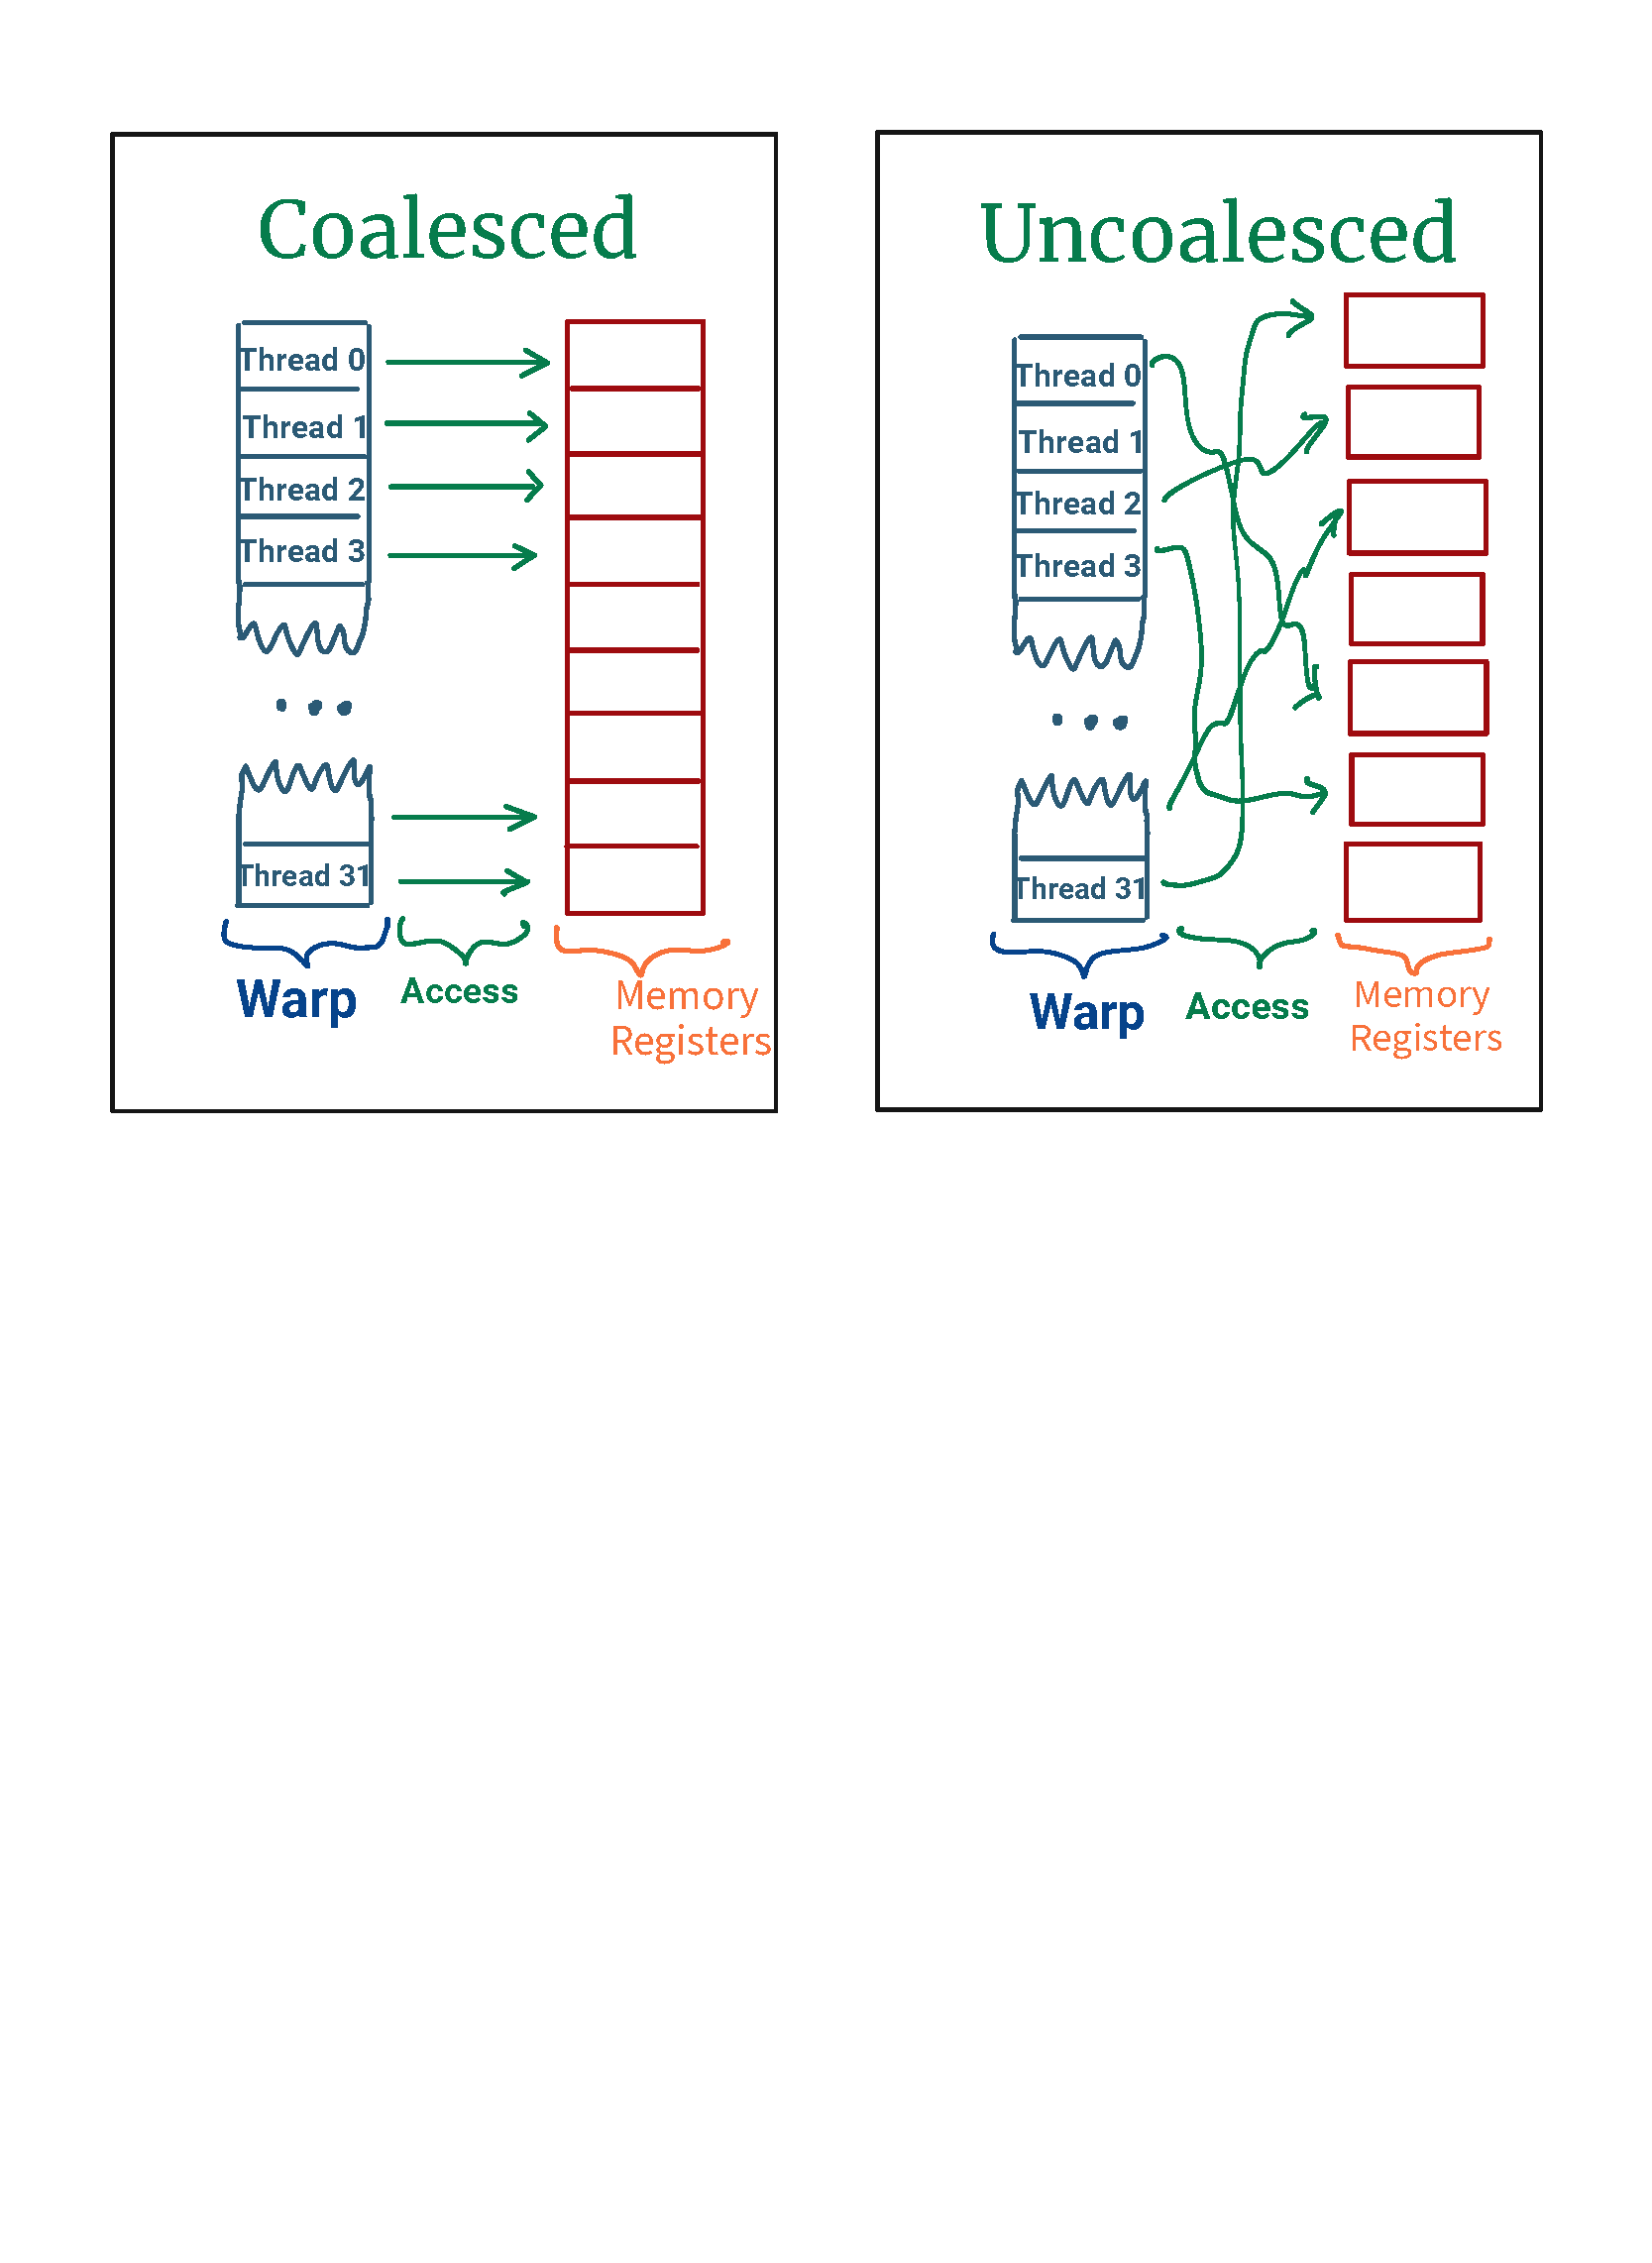
\includegraphics[height=5cm]{pngs/coalesced.png}
    %\end{center}
   \caption{Memory access optimization mechanism.}
   \label{coalesced}
\end{wrapfigure}

Imagine a certain number of warps are scheduled by the SM. Lets say 2 blocks of 128 threads, which gives 
$2\text{blocks}\cdot\nicefrac{128\text{thr.}}{32} = 8 \text{warps}$. These warps fetch some data 
from a certain field of memory of the GPU. We know that the warp is something very grouped, even physically 
the threads are grouped in it. It would be logical that they access adjacent memory addresses. This notion 
may seem quite confusing in the beginning, but let's see how Nvidia is describing it\cite{center}:

\vspace{-10pt}
\begin{quote}
   \textsl{Global memory instructions support reading or writing words \footnote{Words can be data type of a certain size.} 
   of size equal to 1, 2, 4, 8, or 16 bytes. 
   Any access (via a variable or a pointer) to data residing in global memory compiles to a single global memory 
   instruction \textbf{if and only if} the size of the data type is 1, 2, 4, 8, or 16 bytes and the data is naturally aligned 
   (i.e., its address is a multiple of that size). If this size and alignment requirement is not fulfilled, the access 
   compiles to multiple instructions with interleaved access patterns that prevent these instructions from fully coalescing.}
\label{coalescedquote}
\end{quote}
Do not pay attention to the notion of \textbf{global} memory (we will discuss it soon).
Try to read the Nvidia standart above again by looking at the coalesced scheme (\autoref{coalesced})
to fully understand the mechanism. One may notice that this notion is crucial in the performance of the code.
Indeed, when writing the kernel, one must keep in mind this aspect and try to ensure (\sout{when possible}) 
a coalesced memory access.

\vspace{-15pt}
\paragraph{\underline{Global memory}} is the largest memory in terms of the size, and yet with the greatest latency.
As we've discussed, the kernels are launched \textbf{from} the CPU. It would be wise to be able to share 
resources between the host and the device. For example, send data to the GPU from a usual \verb|C| programm
and retrieve back in a processed form. This is exactly the purpose of the global memory. The global memory, as the 
name suggests is \textsl{global}, i.e. it is \textbf{visible to all threads from all blocks}. As we will see in practice,
the usual workflow is to copy the data from the global memory to some other (which is discussed below), 
which is faster \footnote{You may think of it as the {\fontfamily{pcr}\selectfont malloc()} or {\fontfamily{pcr}\selectfont calloc()} functions in C
or the keyword {\fontfamily{pcr}\selectfont new} in C++. Indeed, the allocation and the access to those variables is slower than 
declaring on the stack:\newline {\fontfamily{pcr}\selectfont int $^{\ast}$ ptr\_a = new int; } is slower than {\fontfamily{pcr}\selectfont int a = \{\};}}  
to manipulate. 

\vspace{-15pt}
\paragraph{\underline{Shared memory}} \label{grocery_store} is much faster than the global one, but evidently smaller. Other 
crucial difference is the scope - the shared memory is \textbf{only seen by threads in the same block}. This provides 
the ability for threads to share results and temporary calculations, and process the data \textsc{in place}. 
Think of this situation as a client of a grocery store, where the customers are sort of threads. Every time a person 
wants to cook something at their house, they don't drive to the store to buy every ingredient. They rather go there 
once a week, for example, and buy the amount they need. They also make sure, 
that everything can fit in the fridge. Thus 
in this \sout{wonderful} analogy, the fridge is the low latency shared memory, and the grocery shop - the 
big and unwieldy global resource.
One sometimes refer to this memory as 
\textsl{cache memory controlled by the programmer}. However, it is important to take note that the reduced 
latency of the shared memory does not guarantee a better performance. Indeed, the biggest pitfall for all \sout{of us} beginners 
are the \textit{bank conflicts}\footnote{A small disclaimer: the notion of \textit{bank conflicts} was one of the reasons for these personal 
notes. The reader should not panic if he's missing something. The examples will be discussed later in the practice part. So one 
should, if necessary, come back to this "theoretical" part after going through the examples. \sout{The author wants to apologize 
for the eventual wordiness.}}. 

\paragraph{Bank conflicts.}We already discussed the notion of warps, as an execution entity encapsulating threads. 
One may think of the \underline{bank conflicts} as the analogy of warps in memory
 (i.e. warps are located at the \textit{execution level abstraction}, and the 
 bank conflicts-at the \textit{memory level abstraction}). 
 Shared memory is organized into \underline{banks}.
One \textit{layer bank} is a sequential field of 32 memory adreses of 4 bits ($32\text{\#adreses}\cdot 4\text{bits}$). 

\begin{quote}
   \textsl{Memory can serve as many simultaneous address as it has banks.} 
\end{quote}
This is a very important property, so lest's consider an another \sout{illustrative} analogy. Suppose in a restaurant, each waiter 
is assigned a strict number of tables, such that a waiter $A$ cannot take $B$'s tables. Suppose you are the host at this restaurant, 
and you have a large group of people, who's number is the exact number as the resaurant's seats. The wise choice would be to 
partition them between all the waiter's assigned tables, right? Wouldn't that be silly to partition all the guests, excepting one, 
who will be waiting for a free place at $A$'s waiter's table, while there are free places at $B$'s table? The analogy \sout{may} not be 
the best, but the sketch should do the trick: 

\begin{figure}[H]
   \centering
   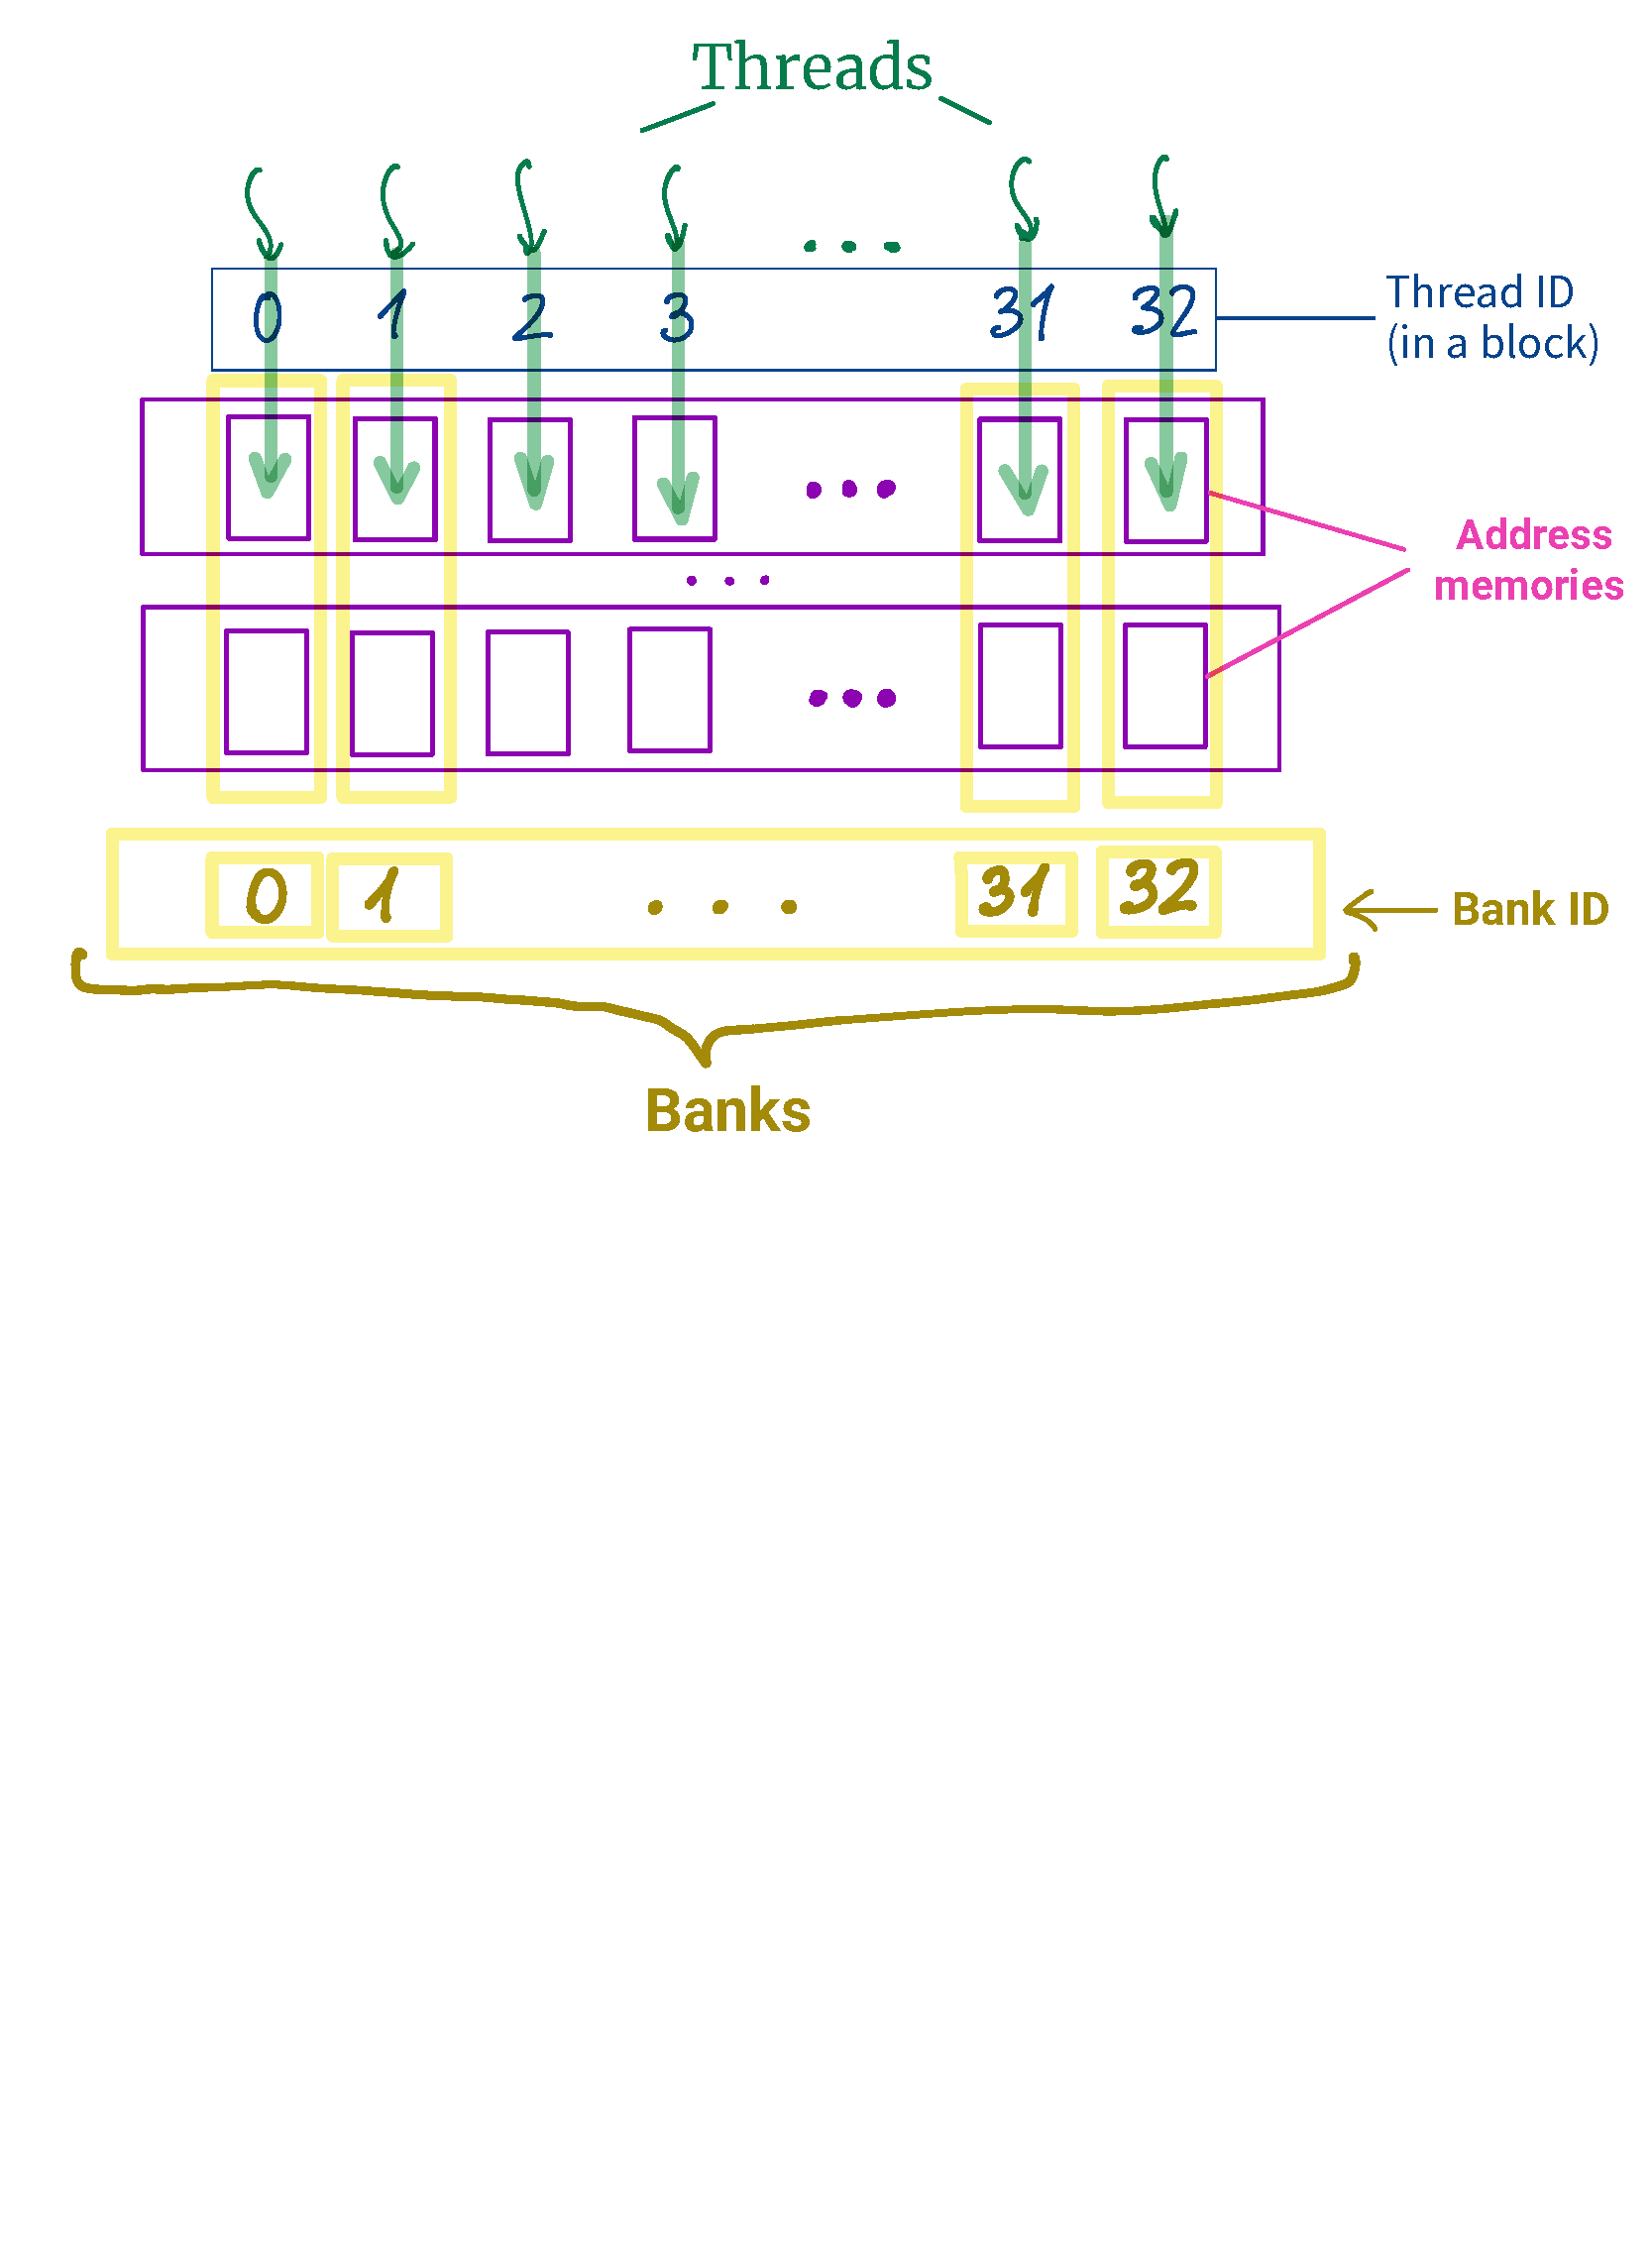
\includegraphics[scale=0.18]{pngs/banks1.png}
   \caption{Memory banks serving the threads. Only one thread can access a bank with a certain ID simultaneously. 
   From the analogy, threads are clients, and banks are waiters, giving them memory.}
   \label{banks}

\end{figure}

\vspace{-0.5cm}
\paragraph{Read-only memory$\ast$} is, as its name suggests, can't be changed by the kernel's threads, but is loaded at compile time. This memory is not as commonly 
described in the GPGPU programming documentation. It is often 
encapsulated in the GPU APIs, such as OpenGL. Thus by using those API's, the programming is indirectly 
reffered as the read-only memory.

\paragraph{Local registers}By looking at the scheme of the architecture of the GPU vs the CPU (\autoref{cpuvsgpu}), one may notice the amount 
of registers in the GPU vs the CPU. The amount of registers in the GPU
is incomprarble with the registers of the CPU. As you might have guessed, a 
register is memory, with the scope of a thread. The compiler of a CUDA program will try to optimize the number and size of registers. 
It is nevertheless possible, that the amount of memory in registers may fall short. Then the L1 and/or L2 caches will enter the 
play. This is the fastest memory available in the CUDA API, yet the most restrictive.

\subsection{Memory allocation model}
\label{subsection:mem_alloc_model}
By now, we've made the difference between kinds of memory in terms of the scope, i.e, 
\textbf{who} and \textbf{when} is able to access various kinds of memory. This, of course, somehow impacts the way we're allocating it. 
However, one can classify the memory, in terms of its \textbf{allocation}. There are mainly fours ways of memory allocation.


We will see further that standart 
code, which uses GPU resources, follows a certain path/pipeline. 
Roughly that is: 
\begin{enumerate}
\setlength\itemsep{-0.1em}
  \item Resource declaration on the host (using \verb|malloc|) and initialization using \verb|memcpy|.
  \item Memory allocation and initialization on the device.
  \item Memory copying/transfer from the host to device.
  \item Accelerated computation on the GPU and storage of the results fro the device
  \item Copy of data from the device back to the host.
\end{enumerate}

One of the steps is the allocation of 
memory on the GPU from the host (by calling a certain CUDA function, which will be described later). 
\begin{itemize}
\setlength\itemsep{-0.1em}
   \item Pageable memory
   \item Pinned memory
   \item Mapped memory
   \item Unified memory
\end{itemize}
The difference in terms of the API calls, use cases and mechanisms, will be explained further. 


















\newpage
\section{Programming in CUDA}

\paragraph{} By now, we have talked about the architecture of the GPU \footnote{Mainly about the Nvidia's architecture, but it 
can be quite well generalized to other GPU's.} by briefly discussing different notions - 
the execution model of threads and kinds of memory. Now, we will try to look at examples of CUDA codes and programs. 
We will try to refer to 
all these prior concepts to get a more detailed understanding. One may need to have a look at the section above 
to link the theory with the practice discussed here. I will do my best to choose the most illustrative examples (of those available 
in different resources) to explain specific concepts, 
as well as introduce some tools. 
Also, note that I use Linux. (\autoref{disclaimer}).

\subsection{Setup}
Before starting to write some code, we must install the necessary packages and libraries. Every computer and operating system 
has its own subtleties, so the best way to install necessary tools, one should check the documentation for the specific system
\footnote{See the installation methods and required components on \url{https://docs.nvidia.com/cuda/cuda-installation-guide-linux/index.html}.}.
For Linux, the main packages are \verb|CUDA| and \verb|CUDA-toolkits|. If we've already used our computer for some time,
we probably have Nvidia drivers installed. 



When we run a \verb|C| program, we need a compiler - arguably, the most common one \sout{and the best one} is \verb|gcc|. For \verb|C++|, 
we invoke his \textit{improved} version \verb|g++|. For CUDA programs, however, we need NVidia's CUDA compiler -
\verb|nvcc|. As we've discussed, the program 
consists of the host and device codes. The device code is just plain \verb|C|/\verb|C++| code, so \verb|nvcc| is also able 
to compile plain \verb|C|/\verb|C++|code. Note that the CUDA code has a \verb|.cu| extension.

\begin{listing}[!ht]
\begin{minted}[frame=single]{zsh}
   $nvcc -o main main.cu
   $./main
\end{minted}
\vspace{-0.7cm}
\caption{Compiling with nvcc and launching a CUDA program on Linux}
\label{nvcc_cuda}
\end{listing}

\vspace{-0.4cm}
If both of the programs do not return an error, the code has been compiled and launched successfully.

\subsubsection{Hello from CUDA}
Let's create our first CUDA and C++ program, and discuss every step below. 
\begin{minted}[frame=single, linenos=true]{cuda}
#include <stdio.h>   //for printf()
#define N_THREADS 4  //number of threads
#define N_BLOCKS 2   //number of block

__global__           //declaration specifier 
void hi_from_gpu(){  //kernel
    printf("Hi from GPU\n");
}
int main(){
    printf("Hi from CPU\n");
    hi_from_gpu<<<N_BLOCKS,N_THREADS>>>();   //invoking kernel
    cudaDeviceSynchronize();                 //synchronize CUDA program
    return 0;
}
\end{minted}

In the output of the following code, we \sout{should} get first \verb|Hi from CPU|, 
followed by 8 times \verb|Hi from GPU|. Let's discuss some aspects of the above code.
Line $5$ contains \verb|__global__| declaration specifier which tells 
the compiler that the following kernel (function) can be launched on the device.
In \verb|main()| function, on line 11, we call the kernel. This is the semantics to 
invoke a CUDA kernel. The \textit{arguments} in the angle brackets \verb|<<<,>>>| 
are the dimension of threads blocks respectively that the kernel will be run on\footnote{We will see further, some additional stuff can be passed
into these brackets, such as the size of memory and streams - concepts that will be seen in further sections
} \& . The type of these dimensions can be either an unsigned integer, or of the \verb|dim3| type, which we will mention in a moment. In this case, 
the GPU will call $2$ blocks, with $4$ threads each. This indeed results in 
$8 = 2\cdot 4$ invocations of \verb|printf()|. Finally, from the main function, we call 
the \verb|cudaDeviceSynchronize()| method, waits for all blocks before the main 
function returns.


\subsection{Threads \& blocks indexing}
Now let's dive in deeper, and access threads and block indexing by modifying our 
\verb|hi_from_gpu()| function:
\vspace{-0.5cm}
\begin{minted}[frame=single]{cuda}
#define N_THREADS 4
#define N_BLOCKS 2
__global__ 
void hi_from_gpu(){
    printf("Hi from GPU\n, from thread id %d and block id %d", 
    threadIdx.x, blockIdx.x);
}
\end{minted}
The output after executing from \verb|main|,
\vspace{-0.5cm}
\begin{minted}[frame=single]{zsh}
   $./main
   Hi from GPU, from thread id 0 and block id 0 
   Hi from GPU, from thread id 1 and block id 0 
   Hi from GPU, from thread id 2 and block id 0 
   Hi from GPU, from thread id 0 and block id 1 
   Hi from GPU, from thread id 1 and block id 1 
   Hi from GPU, from thread id 2 and block id 1 
\end{minted}
\vspace{-0.5cm}
We thus discovered how to access block's and thread's id's. The 
variables \verb|threadIdx| and \verb|blockIdx| are of type \verb|dim3|,
which is a simple structure, containing 3 unsigned int's. By accessing 
its \verb|.x| member variable, we are reffering to the 1D indexing. In general, 
threads are indexed using \verb|dim3| type. Thus, for a thread, living inside a block, there exist x, y and z 
dimensions. And same for the blocks, living in the grid - x, y and z components. 
Think of threads, 
We can launch many threads in many blocks, but how many? This depends on 
the hardware we are using.
To get these specifications, one can look up this information online or ask our computer.\footnote{
To do so, one must find where {\fontfamily{pcr}\selectfont cuda} is located. In my case, it is in 
{\fontfamily{pcr}\selectfont /opt/cuda/}.
Once here, we seek for {\fontfamily{pcr}\selectfont /samples/1\_Utilities/deviceQuery/} 
(or something similar). 
From here, we execute {\fontfamily{pcr}\selectfont ./deviceQuery}.   
}.

\subsection{Memory}

\subsubsection{Vector addition}
The first \textit{useful} example 
that is usually introduced in CUDA tutorials is the vector addition. This exaple
perfectly illustrates the need of GPU parallel model. Indeed, the component of the resulting
 vector $x$ $x_i$ does not depend on other components. So the formula for vector addition is given by 
 $x_i = a_i + b_i$. In sequential execution, we would create a loop, iterate over all elements and 
do something like \verb|x[i] = a[i] + b[i]|. In order to parallelize this workflow, we must initiate $N$ 
threads, with $N = \text{number of components in the vector}$. In \verb|C++|, which simply runs on the host, we create the threads 
using the standart \verb|std::thread|. We know, however, that the CPU does not have many threads (probably from 4 to 12 in most cases). 
This is where the GPU with its multithreaded architecture comes in. The idea here is to launch $N$ threads which are spread over many blocks.
\newline 
To discover memory allocation with code examples, we will consider vector addition. And to do that, 
one must first cover thread \& block indexing for a more general case.

\paragraph{A more complex indexing.} 
We know that the number of threads in one 
block is limited. Let's check on Nvidia's official CUDA documentation \cite{center} concerning threads indexing. 
\begin{quote}
   \textsl{For convenience, {\fontfamily{pcr}\selectfont threadIdx} is a 3-component vector, 
   so that threads can be identified using a one-dimensional, 
   two-dimensional, or three-dimensional thread index, forming a one-dimensional, two-dimensional, 
   or three-dimensional block of threads, called a thread block. This provides a natural way to invoke computation across 
   the elements in a domain such as a vector, matrix, or volume.
   The index of a thread and its thread ID relate to each other 
   in a straightforward way: For a one-dimensional block, they are the same; for 
   a two-dimensional block of size $(Dx, Dy)$,the thread ID of a thread 
   of index $(x, y)$ is $(x + y\cdot Dx)$; for a three-dimensional block of size $(Dx, Dy, Dz)$, the thread ID of a 
   thread of index $(x, y, z)$ is $(x + y\cdot Dx + z\cdot Dx\cdot Dy)$.}
\end{quote}

Before writing some code, let's try to visualize the Nvidia's quote.
\begin{figure}[H]
   \centering
   \includegraphics[scale=0.25]{pngs/tindexing.png}
   \caption{Simple example to illustrate a plain 1D indexing (supposing a block 
   contains 4 threads). We see how the expression \textsc{blockIdx.x*blockDim.x+threadIdx.x} is used (see below). 
   One can easily extrapolate the indexing to 2D and 3D cases, as described in the Nvidia documentation above.
   }
   \label{fig:tindexing}
\end{figure}
Let's now write code to add two vectors, using a 2D indexing \footnote{This is the first and almost the only \textbf{full} example of a cuda program. 
That is, the author will mostly provide the key aspects of the newly introduced features, thus skipping the usual parts of defining things, of allocating 
memory, freeing it, etc.}: 

\begin{listing}
\begin{minted}[
   frame=single,
   framesep=2mm,
   baselinestretch=0.8,
   fontsize=\footnotesize,
   linenos 
   ]{cuda}
#include "stdio.h"
#define N_THREADS 512
#define N_BLOCKS 64 
void init_host_vector(double *a, double *b);
void check_result(double *res);

__global__ 
void add_vec(double *a, double *b, double *res){
    //compute the index
    int id = blockIdx.x*blockDim.x+threadIdx.x;
    if(id < N_THREADS*N_BLOCKS){
        res[id] = a[id] + b[id];
    }
}

int main(){
    const int size_in_bytes =N_THREADS*N_BLOCKS*sizeof(double);
    //initialize the data on HOST
    //malloc() (C) or new (C++) 
    double *hst_a = (double *)malloc(size_in_bytes);
    double *hst_b = (double *)malloc(size_in_bytes);
    double *hst_res = (double *)malloc(size_in_bytes);

    init_host_vector(hst_a, hst_b);

    //allocate memory on GPU
    double* dv_a;    cudaMalloc(&dv_a, size_in_bytes);
    double* dv_b;    cudaMalloc(&dv_b, size_in_bytes);
    double* dv_res;  cudaMalloc(&dv_res, size_in_bytes);

    cudaMemcpy(dv_a, hst_a, size_in_bytes, cudaMemcpyHostToDevice);
    cudaMemcpy(dv_b, hst_b, size_in_bytes, cudaMemcpyHostToDevice);

    add_vec<<<N_BLOCKS, N_THREADS>>>(dv_a, dv_b, dv_res);
    cudaDeviceSynchronize();
    cudaMemcpy( hst_res, dv_res, size_in_bytes, cudaMemcpyDeviceToHost );

    check_result(hst_res);

    cudaFree(dv_res);   free(hst_res);
    cudaFree(dv_a);     free(hst_a);  
    cudaFree(dv_b);     free(hst_b);
    return 0;
}
\end{minted}
    \caption{Basic vector addition, using sequential thread indexing. \cite{tuomanen2018hands}}
\end{listing}

Ok, there are multiple aspects to discuss...

First let's discuss the code. First on the device. Remember we discussed the global GPU memory. 
The line 31 we're working with memory. The classical pipeline of any CUDA program
execution, is usually the following:

\begin{enumerate}
\setlength\itemsep{-0.5em}
   \item Begin code on host.
   \item Allocate memory on host.
   \item Allocate memory on device.
   \item Calculations performed on the device.
   \item Host treats the data.
   \item main() gets returned.
\end{enumerate} 

\paragraph{Allocate memory on host.} To allocate memory on the host, 
we proceed with the usual C \verb|malloc()| function and naturally 
casting the returned pointer to \verb|double*| (don't forget 
to free memory at the end by \verb|free()| function). 
Then we call a simple function \verb|init_host_vector()| that will just initialize the data 
to some values, let's say to simple $0,1,2,3, ...$. 
\paragraph{Allocate memory on device.} Then we allocate \textbf{global memory} on the GPU, 
by calling the \verb|cudaMalloc()| function. Note the arguments that this function takes - 
a \textbf{pointer to pointer} - \verb|(<type> **)| and the size in bytes. 

 
\paragraph{Data copying} between the host and the device is done using the \verb|cudaMemcpy()| function. Also, pay attention 
to the parameters - 
\verb|cudaMemcpy(void* destination, void* source, size_t size_in_bytes,| \newline \verb|enum cudaMemcpyKind kind)|,
with \verb|kind| \footnote{Here, I described the parameters in details. However, further on,
the author will not be that precise. The reference for this function was taken from 
\url{http://horacio9573.no-ip.org/cuda/group__CUDART__MEMORY_g48efa06b81cc031b2aa6fdc2e9930741.html}. 
For further function descriptions, always have a look at it.}
specifying how to copy. In code, it is understandable that the destination is the 
device and the source is the host.

\vspace{-0.8cm}
\paragraph{Calculation.} The kernel computes the sum of a vector of size $512\cdot 64 = 32768$. 
Therefore $64$ blocks of $512$ threads are launched, and $32768$ threads independently execute the \verb|add_vec()|
function. In the kernel, a unique ID is assigned to the thread(line 10) (see the indexing \textit{policy}  see \ref{fig:tindexing}). 
The ID's span from $0$ to $32768$, without ever repeating themselves and covering all the numbers in the interval.
We also add a simple \verb|if()| statement, to be sure, that the thread's ID does not exceed the size of the vector.
Thus every thread does exactly one calculation \footnote{Of course, without taking into account the calculation of the id.}.
Remember that the memory, in which these processes are happening, is the global memory. 

\vspace{-0.8cm}
\paragraph{Terminating.} After the kernel, we call the usual synchronization function, which will, as usual, wait for all the threads and blocks 
to finish the calculations. 
Then, a simple check function on the host, simply to ensure, that the parallel vector addition was successful and that we've received the correct result.
And finally, the \verb|cudaFree()| method, does exactly what is expected - 
frees the allocated memory on the GPU, the exact same things, as the \verb|free()| does in a usual \verb|C| code.

Let's also try to link this piece of code to the section about warps. Remember, 
threads are scheduled by the SM into warps - groups of 32 threads (\autoref{warps}). 
In this case, we're launching a total of $\nicefrac{512}{32} = 16 \text{warps}$ for each 
block, and 64 independent blocks. While working with CUDA threads, it is advised to work with 
the number, which is a multiple of $32$ (the thing we've done in this example). Indeed, imagine, if we were to launch $513$ threads on a block.
Then the SM would schedule 17 warps. This number of warps is the same as if we would launch $544$ threads in a block.
Indeed, this will launch $16\cdot 32 = 512$ threads (executed simultaneously in one warp) \textbf{and} 
one additional thread on an almost empty/unoccupied warp. 

One could also be interested in the difference in the execution time between 2 different
 configurations - either $64\text{threads}\cdot 512\text{blocks}$ or $32\text{threads}\cdot 1024\text{blocks}$
 The benchmarking is very important and useful in GPGPU programming. Different tools and techniques for  
 benchmarking CUDA programs will be discussed in further sections.

\subsubsection{Multiple dimension memory}
By now, we've looked into the global one-dimensional 
memory allocation (and copying) on device. Suppose you would like to work 
with 2D allocated memory. It is clear that we could work without the ability to explicitly allocate 2D or 3D arrays. 
Indeed, if we want to work with, let's say, a 2D matrix, we could simply 
transform it into a 1D vector of size rows$\cdot$cols.
However, there is a feature in the CUDA API, that lets us to allocate 2D, and even 
3D memory \cite{MemoryAlignment}. 
The method that implements 2D memory allocation is \verb|cudaMallocPitch| with the following signature:


\begin{minipage}[h]{0.5\textwidth}
   \vspace{-1cm}
     \begin{minted}[frame=single,framesep=2mm]{cuda}
cudaMallocPitch( void** devicePtr,
                size_t* pitch,
                size_t widthInBytes,
                size_t height);
     \end{minted}
     \captionof*{figure}{The signature of function. Some new terminology 
     given on the \hyperref[fig:pitch]{right}.}
\end{minipage}
\begin{minipage}{0.4\textwidth}
   \hspace{0.2cm}
\includegraphics[scale=0.10]{pngs/pitch.png}
\label{fig:pitch}
\hspace{1cm}
\end{minipage}

This function is allocating \textbf{at least} width$\times$height bytes array
As we have seen, the allocation on the device is followed by the data copy from 
the host. There is also a special function to do so - \verb|cudaMemcpy2D()|. Apart from allocating 
and initializing the device data, we should be able to access it. So let's consider a code snippet
that does so:

\begin{listing}[!ht]
\begin{minted}[frame=single, framesep=1mm]{cuda}
int main(){
   float *A, *dA;
   size_t pitch;
     
   A = (float *)malloc(sizeof(float)*N*N); // allocate on host
   cudaMallocPitch(&dA, &pitch, sizeof(float)*N, N); // allocate on device

   //copy memory
   cudaMemcpy2D(dA,pitch,A,sizeof(float)*N,sizeof(float)*N, N,\
      cudaMemcpyHostToDevice);
         /*...*/
}
__global__ void access_2d(float* devPtr, size_t pitch,\
            int width, int height) {
    for (int r = 0; r < height; ++r) {
        float* row = (float*)((char*)devPtr + r * pitch);
        for (int c = 0; c < width; ++c) {
            float element = row[c];
        }
    }
}
\end{minted}
\caption{To get this straight, one should know 2D array work in pure C. 
  Indeed, to access an element, we first identify the current row, by doing some pointer manipulations. 
  And then, once the pointer to the very beginning of the row is identified, we iterate over this 
  row, by accessing it sequentially. Also note that in the code, in order to identify the 
  row for the next iteration (i.e. it's $0$'s element pointer), one uses the size of the pitch, and 
  not of the width. We see that this 2D pitch is allocated 
    \textbf{automatically} by the CUDA memory management system \cite{blog_2020}
  }
\label{allocation2d}
\end{listing}


As you might have guessed, this memory access is not extremely efficient. As one may say, \textsc{this is for educational purposes only}. In the documentation, it is recommended 
to use these functions to allocate and initialize the 2D memory on device. Hopefully, we all can find 
use cases of this memory and efficient indexing \footnote{There are a lot more of memory allocation, \& memory copy methods, 
provided in the CUDA API. For example {\fontfamily{pcr}\selectfont cudaMallocArray()}, which has also a different signature.
The different methods, dedicated to memory allocation and management can be observed \url{https://courses.cs.duke.edu/cps296.3/fall09/cuda_docs/html/group__CUDART__MEMORY_ge56101fe6f1ce0b48f163632f6862ae4.html#ge56101fe6f1ce0b48f163632f6862ae4} }.

\subsection{More on Memory}
\subsubsection{Shared memory vs global memory}

For now, in the examples, we've only looked into the global (\& pinned) memory. It is global and accessible 
for all threads in all blocks for both read and write operations, and yet having high latency, compared to 
more local memory types, such as the shared one. Shared memory's scope is one \underline{thread block}. Thus, if, let's say,
a block contains 16 threads, the shared memory can only be read and modified by 16 local threads. If one wants to operate on it 
locally, the data must be copied to it. Therefore, if one wants this memory to be accessed/modified by 2 thread blocks ($=32$ threads), one 
must make sure that the data has been copied to the shared memory of the two blocks.

Let's now consider a more complex and yet classical example - matrices. Recall basic matrix operation - 
\begin{itemize}
   \setlength\itemsep{-0.5em}
   \item If $A$ - $m\times n$ matrix ($m$ rows and $n$ columns), it can be added to some 
   other matrix $B$ of same size $m\times n$, by adding element-wise each element $a_{i,j}+b_{i,j}$. 
   \item One can multiply two matrix $A$ and $B$ - $C = A\cdot B$ by using the formula 
   $c_{i,j} = a_{i,1}\cdot b_{1,j} + a_{i,2}\cdot b_{2,j} + ... + a_{i, n}\cdot b_{j,n}$, only if the matrix 
   $A$ is of size $m\times n$ and $B$ of size $n\times p$. In short, the resulting 
   element $c_{i,j} = \sum_{k=1}^{k=n}a_{i,k}\cdot b_{k,j}$ and yields $C$ of size $m\times p$.
\end{itemize}

One can perform these operations using the global memory, or shared memory.

\paragraph{Global} version code snippet is given down below.


\begin{listing}
\inputminted[linenos=true, frame=single]{cuda}{cucodes/matmulglob.cu}
    \caption{Basic, yet important, global memory usage. \cite{tuomanen2018hands}}
\end{listing}

Before moving to the code discussion, let's make a small \textit{intermezzo}
on transforming 2D array to 1D, to make things clear and easier for further analysis:

\noindent\fbox{
   \parbox{0.96\textwidth}{
   Suppose we are given a 2D array (matrix). But we know that, behind the scenes,
   (even if we're accessing a[i][j] in many programming languages), it all breaks 
   down to contiguous, linear memory addresses. So suppose you have allocated 
   a 1D array arr of size $N$. The, you could access your i'th element by doing {\fontfamily{pcr}\selectfont arr[i]}  
   (supposing C or C++) or by doing {\fontfamily{pcr}\selectfont*(arr + i)}, where 
   {\fontfamily{pcr}\selectfont arr} - the address of the 0'th element 
   of the array . So the formula is given by $\text{A}_{i^{th}} = A_{0} + \text{sizeof(type)}\cdot i$, where 
   $A_0$ - the first (0'th) memory address and sizeof-the size of one memory field (e.g. sizeof(char) = 1).
   Suppose now, that we've allocated a 2D memory array of size $M\text{rows }\times N\text{cols}$. For the first row
   one can apply our previous formula - $A_{0,j} = A_{0} + \text{SZ}\cdot j$. However, if $j$ is 
   greater than $N$ - the number of columns, a problem occurs. If we work in 2D indexing, over a loop, we would just 
   \textit{reset} our index $j$ to 0 and increment $i$ (if $j=N-1$). However, in a flattened 2D case, in order to 
   access $A_{i,j}$ address-wise, we use the expression 
   $A_{i,j} = A_{0} + \text{sizeof(type)}\cdot N\cdot i + j)$. One can easily check, that this expression is consistent with all the 
   examples. This expression is for row-major arrays - accessing successive elements in a certain row.
   }
   \label{intermezzo1d2d}
}
\vspace{1cm}


Okay, now we can attack the code. From line 13 to 21, we are initializing the data and 
allocating memory. The lines 27 \& 28 are initializing the dimensions 
(number of threads in x,y directions and the number of blocks in the x, y directions), that the kernel will be launched on. 
Note that we are using 2D indexing for the first time.
In this case, \verb|grid_dim| is the dimension of the grid, 
in which blocks are contained. The \verb|block_dim| is the block dimension - the number of threads in the block. 
In this case there are $16\cdot 16 = 256\text{threads}$ and $\frac{32}{16}\cdot \frac{32}{16} = 2\cdot 2 = 4 \text{blocks}$. 
So there are $256\cdot 4 = 1024 \text{threads}$ partitioned between 4 blocks. This is exactly what we need, 
because the resulting matrix $C$ is exactly $32\times 32$, which gives us 1024 elements. Therefore, if everything goes well,
each thread will perform the calculation for each element $c_{i,j}$ of the matrix $C$. 
In theory, we would like that 
each thread iterates over one line of the matrix $A$ and one column of $B$. Remember the \hyperref[intermezzo1d2d]{1D to 2D mapping}. 
is going through all the elements in the row $i$ of the matrix $A$ (line 43). 



\vspace{-0.9cm}
\begin{gather*}
 A_{i, h} = A_{0} + i\cdot N_{cols(A)} + h
\\
B_{h,j} = B_{0} + h \cdot N_{cols(B)} + j
\end{gather*}
These equations (at least the first one) are exactly predicted by \hyperref[intermezzo1d2d]{1D to 2D mapping} and
are represented on the lines 43 and 44 of the code snipped. 
Finally, once each thread runs over its own row and column, it is 
gathering the result by assigning this accumulated sum to the 
\verb|C[i][j] = C[i*Width + j]|, where i,j - row id's and column id's respectively\footnote{This 
aspect is not simple yet basic. This is a common CUDA pattern, which needs to be understood correctly 
\sout{(or at least know where to look for)}. So one should try to visualize the indexing process and the algorithm workflow. }


\paragraph*{Shared memory} is one of the key, to control the efficiency of a CUDA program. 
As we've mentioned several times before, the shared memory is only visible in the block's scope. That means that 
if, we would want to make the shared memory visible \& accessible to all threads in the entire kernel, we would 
need to allocate (and transfer the data to) shared memory, which belongs to independent blocks. 
Remember the analogy of the \hyperref[grocery_store]{grocery store}.
It's up to the programmer to decide, whether it would be reasonable to spend time on algorithm design, using shared memory, and its allocation
 (which, of course, takes time, but has little latency, when using it), or to high-latency global memory access.
So let's have a look at a shared memory code snippet\footnote{For space-saving's sake, only a snipped is provided. The skipped pieces are usual steps of 
memory allocation, freeing resources, etc...}.
demonstrating shared memory usage for matrix multiplication. 
Let's first discuss the general strategy. As we have said, the shared memory is much smaller in terms of size 
than the global one. So here, the main idea is to divide the \textit{big} matrices $A$ and $B$, that we're multiplying into smaller
sub-matrices, which will be loaded into the shared memory later of each independent block.

\begin{figure}[ht!]
   \centering
   \includegraphics[width=0.6\textwidth]{pngs/globalmatrix.png}
   \vspace{-0.5cm}
   \caption{Scheme of 2D matrix multiplication, using Shared memory}
   \label{global2d}
\end{figure}


Let's look at the code describing this strategy:

\begin{minted}[frame=single, framesep=1mm, linenos=true]{cuda}
typedef struct{
   int width; int height; int stride;
   float *elements;
}Matrix;

__device__ float GetElement(const Matrix D, int row, int col)
{
    return D.elements[row * D.stride + col];
}

__device__ Matrix GetSubMatrix(Matrix D, int row, int col) 
{
    Matrix sub;
    sub.width    = BLOCK_SIZE;
    sub.height   = BLOCK_SIZE;
    sub.stride   = D.stride;
    sub.elements = &D.elements[D.stride * BLOCK_SIZE * row
                                         + BLOCK_SIZE * col];
    return sub;
}

 __global__ void mult_global(Matrix A, Matrix B, Matrix C)
{
    // blockRow & blockCol (see image)
    int blockRow = blockIdx.y;
    int blockCol = blockIdx.x;

    // Create Csub, initial matrix
    Matrix Csub;
    Csub = GetSubMatrix(C, blockRow, blockCol);
    float Cvalue = 0; //we will accumulate values (see figure above)

    // Thread row and column within Csub
    int row = threadIdx.y;
    int col = threadIdx.x;

    // Loop over all the sub-matrices of A and B 
    // Multiply each pair of sub-matrices together
    for (int m = 0; m < (A.width / BLOCK_SIZE); ++m) {//iterate over 
                                          //sub-matrices//of A(see fig above)  
        Matrix Asub=GetSubMatrix(A, blockRow, m);//Asub of A(m-the index of row)
        Matrix Bsub=GetSubMatrix(B, m, blockCol);//Bsub of B(m-the index of col)

        // shared memory to store Asub and Bsub
        __shared__ float Asub[BLOCK_SIZE][BLOCK_SIZE];
        __shared__ float Bsub[BLOCK_SIZE][BLOCK_SIZE];

        // Each thread loads one element of each sub-matrix Asub and Bsub
        As[row][col] = GetElement(Asub, row, col);
        Bs[row][col] = GetElement(Bsub, row, col);

        //All threads must be synced, to be sure all data is loaded properly
        __syncthreads();

        // Use matrix multiplication formula to get the Csub element
        for (int e = 0; e < BLOCK_SIZE; ++e){
            Cvalue += Asub[row][e] * Bsub[e][col];
        }

        __syncthreads(); //synchronize before new sub-matrices are loaded
    }
    C.elements[row * A.stride + col] = Cvalue;
}
   int main(){
      /*init matrices on host
      * init matrices on device with cudaMalloc(),
      * copy data from host to device
      */
   dim3 dimBlock(BLOCK_SIZE, BLOCK_SIZE);
   dim3 dimGrid(B.width / dimBlock.x, A.height / dimBlock.y);
   mult_global<<<dimGrid, dimBlock>>>(d_A, d_B, d_C);
   }
\end{minted}

Okey, let's now discuss in detail the execution of the kernel \verb||, and try to make as more analogy as possible
with the scheme above.
\begin{enumerate}
   \item The matrices are assumed to be multiples of BLOCK\_SIZE (block dimension in fact). In this case, let's say $32\times 32$. So, 
   from the main function, we're launching 32 threads in each block, and $2\times 2 = 4$ blocks in a grid. Thus we have 
   $32\times 32\times 4=4096 \text{ threads}$, organized in a grid of 4 blocks. So there is a kind of mapping between 
   the 2D matrix and the threads partitioned into blocks.
   Keep that launched chunk of threads in mind. 
   \item The first thing we do in the kernel is attribute the block row and column ids. They correspond to blockRow and blockCol, 
   annotated in the figure \ref{global2d}. There will thus be 4 sub-matrices to which, to which each block will be assigned to (as we've said 
   that the block is of size $16\times 16$ and the matrix size is $32\times 32$). Remember that
   the shared memory is \textbf{only visible inside a block}. Thus the possible configurations of the indices are given by 
   $(A_{row}=0, B_{col}=0)$, $(A_{row}=0, B_{col}=1)$, $(A_{row}=1, B_{col}=0)$ and $(A_{row}=1, B_{col}=1)$. These indices correspond to the 
   \textit{olive color} strips on the figure, labeled with BlockRow and BlockCol respectively.
   \item Then we're initializing the sub-matrix $C_{sub}$ - its dimensions, elements and stride.
    The stride, in our case, is the offset we need to take into account when computing the elements in the row-major form. Note that it is not always
    the same as matrix width. For example, when we're dealing with the submatrix, the stride does not equal to its width, but rather 
    \textbf{the original matrix width}. Indeed, the size of the submatrix does not affect the element's addresses in memory.
    This sub-matrix $C_{sub}$ is illustrated in figure \ref{global2d}. 


        This gives us the ability to keep 
   track of the sub-matrix within each block. Remember, the multiplication 
   of (sub-)matrices involves the accumulation of element-wise multiplication, so we're initializing the temporary sum to $0$.
   \item The initialization is followed by the initialization of sub ids. These are the thread ids \textbf{within a block}.
   Thus these id's will be uniquely identified for each thread within the block, launched on a unique kernel instance. And, as we know, each block will be responsible 
   for one sub-matrix of $C$ - $C_{sub}$. These ids are represented by yellow rows and columns on figure.
   \item Now, an important assumption will be made - the number of blocks contained in A's matrix width is the same as the number of 
   blocks contained in the B's matrix height\footnote{This is an assumption, that is, as we say W.L.O.G - without loss of generality. 
   Indeed, if this assumption is not the case, one could modify a bit the code for it to work without this assupmtion.
   However, this is neither a problem, because, one can allocate and perform operations on a bit bigger matrices, without big issues in 
   performance}. This is the reason why we can use the first loop, to iterate over A'th width and B'th height \textit{simultaneously}. 
   \item As mentioned just above, we can simultaneously iterate over A'th width and B'th height, thus simultaneously obtaining the sub-matrices 
   $A_{sub}$ and $B_{sub}$. After getting the sub-matrices $A_{sub}$ and $B_{sub}$, we allocate shared memory \verb|As| and \verb|Bs| for 
   $A_{sub}$ and $B_{sub}$ using the \verb|__shared__| directive. Note here, that each thread in the block is retrieving \textbf{one, and only one element} of the matrix. 
   Indeed, the \verb|getElement()| method retrieves only one element from global to local memory. This is the most important step in this 2D matrix multiplication.
   \item After each thread retrieves the data \textbf{within the block}, we would like all threads to be done with synchronization. Indeed, in global memory's case, 
   each thread accesses the global memory independently, with a unique ID. Here, with the shared memory, we introduce a kind of independence between threads, by making them all access to the same block-local shared memory, by 
   making them all retrieve local data. So, for example, suppose we have a $4\times 4$ sub-matrix. Each thread within the block loads one element into shared memory (seen by the other 15 threads). So before 
   making the calculations, we want all the 16 data to be loaded into shared memory.
   \item Afterwards, we are finally doing calculations on the sub-matrix, using the previously retrieved elements of $A_{sub}$ and $B_{sub}$ into \verb|As| and \verb|Bs| respectively.
   Remember here that \verb|row| and \verb|col| are unique for each thread. Once again - This step is illustrated in the figure: the iteration is performed through the yellow 
   line's multiplication element-wise. And the \textbf{unique} elements, attributed to the threads are the \verb|row| and \verb|col| indices. This is the final result 
   we want to achieve: \textit{each thread within the block multiplies the \textbf{row} of $A_{sub}$ and the \textbf{col} of $B_{sub}$ element-wise, to get only one element of the $C_{sub}$ sub-matrix}.
   \item The final step of the kernel is to copy each element of the $C_{sub}$ sub-matrix to the global memory. Once again, 
   as each thread is doing its own $Csub_{i,j}$ element, it is just copying only \textbf{one} element to global memory.   
\end{enumerate}
   Note that apart of the \verb|__shared__| directive, other, new technical aspects were used. First - the \verb|__device__| directive.
   It declares a function, which can \textbf{only} be called from the device function (the one declared with \verb|__global__|). These device functions 
   can return different types. Second - the shared memory with the \verb|__shared__| directive. As discussed above, this is shared memory, only seen within the block.
    

   As mentioned, this is a very fundamental example, yet not simple, and takes time to understand. The reader \sout{and the author} must go through the code 
   and the illustration several times. As well as going through multiple particular instances of the code, with particular instances of the block and threads ids.


\begin{figure}[h!]
   \centering
   \subfloat[\centering]{{\includegraphics[width=7cm]{pngs/bank_conflict.png} }}
   \qquad
   \subfloat[\centering]{{\includegraphics[width=7cm]{pngs/bank_conflict-2.png} }}
   \caption{Bank conflicts}
   \label{fig:bankconflicts2}
\end{figure}

\paragraph{Bank conflicts.} We have practically discussed several applications of the theoretical notions described in the section 
on architecture. How about the bank conflicts? Remember - the warps are chunks of threads (way of scheduling/organizing them). 
The banks are chunks of memory and a way to structure them. Also remember that, ideally, 32 threads, 
organized in one warp, access simultaneously one "column" at a time \autoref{banks}. So if two threads in a warp access simultaneously 
one bank (one column), there is a bank conflict, and the warp will be forced to get split into two execution periods. 
The classical bank conflict is often illustrated by the 2D array initialization in shared memory. 

Once again: suppose we are simply allocating a 1D array (either in global or shared memory) of size 32 bytes. Then one warp is accessing one bank of memory. 
Suppose now we're allocating 64 or 128 bytes of memory, then 2 or 4 warps respectively will access the memory sequentially, i.e. 2 and 4 periods respectively.

So, in order to avoid these bank conflicts in 2D memory (of course, it is always possible to map a 2D array into 1D array, which is much easier to deal with), one should allocate 
\textit{a bit more memory} than required. Take a look at the \autoref{fig:bankconflicts2}: the two first figures (a \& b) show a 1D and 2D array memory access respectively. 
On the LHS, the memory access is a multiple of 32. Therefore, at the same time, more than 2 columns - \textbf{banks}, are accessed by the same warp (multiple of 32). 
In order to get rid of a bank conflict in a 2D memory access, whose size is multiples of 32 (warp's size), we allocate one additional byte to each row (or 4 bytes if it's a float).
To do so, we replace \verb|__shared__ float Mat[BL_SIZE][BL_SIZE]|, with \verb|__shared__ float Mat[BL_SIZE][BL_SIZE+1]|. Indeed, if the addresses are multiples of 32, each warp will 
have to access the same bank/memory address as the previous and the next bank. So, what one can do, is to allocate memory of size 33 rows. Thus, the threads, seeking memory, will 
access different banks(columns).

The author does fully understand and does know that this is a quite subtle aspect, and one needs time to get used 
to these concepts. It is also clear that these things are difficult \sout{or even impossible} to debug and track, once the code is written, and the programmer 
does not have any ideas of where to look for the performance issues. In most cases, 
the \textit{solution} is to simply benchmark the execution of the program, and consequently test the program with different configurations. 

\subsubsection{Other memory addressing}
The main memory, we'll work with is the global and shared memory. However, it would be instructive to have a look at the 
syntax of constant and texture memory allocations. So that, once we come across some of this syntax, we know what is meant 
in this specific piece of code. 

\vspace{-15pt}
\paragraph{Constant memory } is specified with the \verb|__constant__| directive.
Similary as we've done for shared memory with the \verb|__shared__| directive. 
Thus, the constant memory allocation/initialization outside the device code would look something like 
\verb|__constant__ float data[256]|. Now, in the device code, in order to access it, one simply writes \verb|data[i]|.
Now, the next question is how to access this memory from the host code. That is, how to initialize the 
memory from host. To do that, one writes 
 To do that, one writes 
\begin{listing}
\begin{minted}[frame=single, framesep=1mm]{cuda}
//host code
__constant__ float data[256];
cudaMemcpyToSymbol(coeffs, hostData, 256*sizeof(float));
\end{minted}
\caption{Constant memory allocation for device from host. The \textsl{hostData} pointer will be 
the one used in the device code. \cite{talonmies_cudamemcpytosymbol_2013}}
\end{listing}

One can ask ourselves a question on the difference between the mentioned \verb|cudaMemcpyToSymbol()| and \verb|cudaMemcpy()|
functions. The reason, why we can't use the the classical \verb|cudaMemcpy()| function, is because once we declare 
the constant memory using the \verb|__constant__| directive, it has already been explicitly \textit{allocated} and identified as 
constant memory. However, with \verb|cudaMalloc|, we're implicitly assuming, that the memory is global. Therefore, the in order to use 
the \verb|cudaMemcpy()| function, one must first retrieve the address of the constant memory pointer.
For that, we write
\begin{minted}[frame=single, framesep=1mm]{cuda}
//host code
__constant__ float data[256];
float *dcoeffs;
cudaGetSymbolAddress((void **)&dcoeffs, coeffs);
cudaMemcpy(dcoeffs, data, 256*sizeof(float), cudaMemcpyHostToDevice);
\end{minted}
The data can then be used safely from the device.

\vspace{-15}
\paragraph{Texture memory}, as mentioned, will discuss extensively the texture memory. The only 
thing I'll do is to mention, the functions that are associated with the texture memory. The terminology 
for it is similar to the OpenGL's one. That is, vertex buffer objects, vertex array object \cite{noauthor_docsgl_nodate}. Such functions are:

\begin{minted}[frame=single, framesep=1mm]{cuda}
cudaMallocArray() //memory allocation
cudaBindTextureToArray() //memory association with specific texture
\end{minted}

and many others. For more informations : \cite{noauthor_steps3d_nodate}.
%https://stackoverflow.com/questions/16119943/how-and-when-should-i-use-pitched-pointer-with-the-cuda-api

\subsubsection{Memory mapping}
\label{subsub:mem_mapping}
We have discussed multiple kinds of memory - \textbf{Global}, \textbf{Shared}, 
\textbf{thread-local} memories. All of them have different scopes, 
bandwidths, and properties(such as bank access). These memories are classified by their scope, 
not by the way they are allocated and transferred (see \ref{subsection:mem_alloc_model}).

%Until now, we have discussed, that shared memory is invoked with \verb|__shared__| compiler 
%directive. The local memory is thread-local memory, when, for example, we initiate simple memory 
%on stack in a \textbf{kernel}, e.g. \verb|int a = 64| (this \verb|int| a is allocated to each thread's
%register locally). 
%
%The global memory is invoked with \verb|cudaMalloc()| function, called from host. Think of 
%global memory as a \textit{long} transfer between the host and the device. 
%The CUDA API provides, in some ways, to make this process faster. 
%
%
%Note that the following classification is 
%concerning the global memory. \textit{channelling}\footnote{The way the host and the device are 
%communicating with each other, to allocate memory}.
%
%\begin{quote}
%   $\text{HOST}\xRightarrow{\text{owns}}\text{Pageable\& Pinned} \xrightarrow{ALLOCATES}\text{DEVICE}$
%   \label{quote:pinned_pageable}
%\end{quote}

Lets now treat and have a look at different memory allocation types \cite{memory_model}:

\begin{itemize}
   \setlength\itemsep{-0.5em}

   \item \textbf{Pageable data transfer.} When we invoke the \textit{classical} \verb|cudaMalloc()|, 
   we're acessing pageable memory. It is the default behaviour. 
    Under the hood, it is allocated twice - first to pinned memory(see below), 
   then, from the pinned one, to the device global memory. 
      \begin{equation}
        \text{HOST}\xRightarrow{allocates}\text{Pageable} 
        \xRightarrow{} \text{Pinned} \xRightarrow{goes\ to}\text{DEVICE}
      \end{equation}
    One can think of it as the longest path between the host data, 
   and the required device data.
    The syntax for this process is:
    \begin{enumerate}
      \item In order to allocate memory on the host, one uses \verb|malloc()| or \verb|new|.
      \item In order to allocate the memory on the device \verb|cudaMalloc()|.
      \item In order to copy memory from the host to device and vice-versa, one use the \verb|cudaMemcpy()|.
    \end{enumerate}

   \item \textbf{Pinned data transfer} lets us avoid 2-way memory allocation between the host and the device. 
  We are thus skipping one step in the memory allocation pipeline.
   Pinned memory is faster, yet reduces the 
    performance from the host side, as the amount of memory 
    for host processing is reduced.
  The syntax for pinned memory is given by:
    \begin{enumerate}
      \item In order to allocate memory on the host, one uses the \verb|cudaMallocHost()|.
      \item In order to allocate the memory on the device \verb|cudaMalloc()|.
      \item In order to copy memory from the host to device and vice-versa, one use the \verb|cudaMemcpy()|.
    \end{enumerate}

   \item \textbf{Mapped memory}, also called \textit{zero access memory}
     \cite{memory_model}, is pinned memory, which is \textbf{directly} initialized/mapped to the device address. 
    This gives the ability to leverage the device's memory using the host if it is not big enough.
    This also gives a lower memory transfer time. As there is in a way, \textbf{no} memory transfer.
    The syntax for the zero access memory usage is given by:
      \begin{enumerate}
        \item In order to allocate the memory, one uses the \\
          \verb|cudaHostAlloc(void** host_ptr, size_t size, int flags)|, where the flags, e.g. \verb|cudaHostAllocMapped|.
        \item In order to get the communication channel between the host and device, one uses 
          \verb|cudaHostGetDevicePointer()|.
      \end{enumerate}
    You may notice that there is no 2 memory allocations - from the host and device sides. Instead, 
    there is only one memory allocation, and one \textit{pointer sharing}. This emphasizes the \textit{zero mapping}
    fact of the mapped memory.
The flaw of this method is the increase of processing time, as the data is simply mapped, and not copied.

   \item \textbf{Unified memory} is, as its name suggests, memory available both to the host and the device. 
     The biggest advantage of it, is the reduction of the memory allocation pipeline. 
     However, the latency of memory access is highly increased. 
     In order to use and invoke the unified memory, one only uses the \verb|cudaMallocManaged()|. 
     There is no other functions to invoke, as the memory is initialized for both the host and the device.

   \label{mem_alloc}
 \end{itemize}
 Note, that this GPU $\leftrightarrow$ CPU communication is assured via the so-called \textbf{peer access}, 
 which is represented by the \verb|cudaDeviceEnablePeerAccess()| function (see official documentation \cite{center} and \cite{boreskov__nodate}).
  


\subsubsection{Asynchronous memory}
  \label{subsub:async_mem}
  We have seen that both the memory access and memory allocation will affect the program execution time. 
  Therefore when designing a program, one must take into account not only the memory access but also 
  the memory allocation time. 
    The asynchronous memory allocation may reduce the time of program execution, as it is asynchronous. And 
    non-blocking. This concept of asynchronous memory allocation involves the concept of streams discussed 
    further. 
    Therefore the main part of this functionality is discussed in the CUDA streams section \autoref{subsub:async_streams}.
  The asynchronous memory copy is a non-blocking memory copy. The async memory copy is 
  invoked with the \verb|cudaMemcpyAsync()| function. This can be for example used, when one wants to invoke 
  many kernels, with many memory copies. Let's have a look at an abstract example, without going into details, of what is the kernels 
  doing. 
  \begin{listing}
  \begin{minted}[frame=single, framesep=1mm, linenos=true]{cuda}
  for (int i = 0; i < nStreams; ++i){
    int offset = i * streamSize; //offset for memory copy 
    cudaMemcpyAsync(&d_a[offset], &a[offset], streamBytes,\
      cudaMemcpyHostToDevice, stream[i]);
    kernel<<<streamSize/blockSize, blockSize, 0,\
      stream[i]>>>(d_a, offset);
    cudaMemcpyAsync(&a[offset], &d_a[offset], streamBytes,\
      cudaMemcpyDeviceToHost, stream[i]);
  }
  \end{minted}
  \caption{The code snippet \cite{async_memcpy} is giving an example of how to use the asynchronous memory copy. 
Thanks to the streams combination with the async memory copy, the only synchronization that is happening is the memory copy and kernel execution, inside 
a separate stream. That is, if no streams are specified, every iteration is will wait for the previous one to finish. For details, see \autoref{sec:streams}.}
\end{listing}


\newpage
\section{Basic parallel algorithms \& patterns}
\subsection{Reduce}
Consider the situation, when we need to add all the array's elements together. In \verb|C++|, one could use 
the STL algorithm \verb|accumulate()| function. In a more primitive implementation, we would do a single for-loop 
and accumulate the results in one variable. The complexity of such an algorithm would then be about $O(n)$, where 
$n$ - the length of the array. However, one could add some parallelism to this algorithm. 
Indeed, at first iteration, what we would 
do is add the 0th element with the 1st, the 2nd with the 3rd, the 4th with the 5th, etc... Notice that 
all of these $\nicefrac{N}{2}$ additions can be done in parallel (that is, each thread does one addition). The next \textit{iteration} would be 
summing the result of the sum of 0th and 1st with the sum of 2nd and 3rd, thus giving a total of 
$\nicefrac{N}{4}$ additions (instead of $\nicefrac{N}{2}$ ) . 
Therefore, the number of necessary divisions in the next step will be half of those, during the previous ones.
As those divisions are performed in parallel, this algorithm looks like a log-scale complexity. 


\begin{figure}
   \centering
   \begin{subfigure}[t]{0.45\textwidth}
        \centering
        \includegraphics[width=6cm]{pngs/reduce_global.jpg}
        \label{fig:static}
    \end{subfigure}
    \begin{subfigure}[t]{0.45\textwidth}
        \centering
        \includegraphics[width=6cm]{pngs/reduce_shared.jpg}
        \label{fig:dynamic}
    \end{subfigure}
\label{fig:reduce}
    \caption{Reduce algorithm with differnet strategies.}
\end{figure}

\subsubsection*{Global memory reduce}
Let's first have a look at a \sout{not-so-}naive implementation of the discussed reduce algorithm on the GPU.
Once again, we're looking at a simplified version of the code, without implementing memory allocation, copy, etc... 
(note that in this case, we use simple global memory with \verb|cudaMalloc()|). The implementation of this is given by \autoref{listing:global_reduction}.


\begin{listing}
\begin{minted}[frame=single, framesep=1mm]{cuda}
__global__ void reduce_global_kernel(float *data_out,\
               float *data_in, int stride, int size) {
int idx_x = blockIdx.x * blockDim.x + threadIdx.x;
if(idx_x + stride < size){
data_out[idx_x] += data_in[idx_x + stride];
}
}

void reduce_global(float *d_out, float *d_in, int n_threads, int size) {
int n_blocks = (size + n_threads - 1) / n_threads;
for (int stride = 1; stride < size; stride *= 2){
   reduce_global_kernel<<<n_blocks, n_threads>>>(d_out, d_in, stride, size);
}
}

//main()
\end{minted}
    \caption{Global memory reduction. \cite{tuomanen2018hands}}
    \label{listing:global_reduction}
\end{listing}

\begin{wrapfigure}{R}{0.45\textwidth}
   \vspace{-0.9cm}
   \begin{center}
   \includegraphics[width=0.45\textwidth]{pngs/reduce_only_global.jpg}
   \end{center}
   \vspace{-0.5cm}
   \captionsetup{justification=raggedleft}
   \caption{The description of every iteration, for the global memory 
   reuction kernel. Note the how stride is doubling every iteration, 
   ,and how the elements are accumulating in the very first (0th) element of the output data. 
   One should understand, that the code works for arbitrary number of blocks, as we're working with global 
   memory, visible to all threads in all blocks}
   \label{fig:reduced_global_only}
\end{wrapfigure}

Okay, let's discuss the \autoref{listing:global_reduction}. First, in the host function, we define the number of blocks. 
In this case, this number is not so important. It would be important to optimize the execution, 
by taking into account the notion of warps, etc... The important part is the loop in the host code and 
the device kernel. We will try to do the debugger's job and inspect the steps. 
During the first iteration, the value of \verb|stride| is 1. The important point is that the thread id, 
computed in the kernel does not depend on the value of the stride. This is because we're working with the global 
memory, and the access is global.

Suppose the size is $32$, partitioned into 1 block. Then for the first iteration, we'll get, 
\verb|out[0] = [0]+[1]|, \verb|out[1] = [1]+[2]|, ... \verb|out[30] = [30] + [31]|. This is exactly the first iteration, 
shown in \autoref{fig:reduced_global_only} (the case of size=8). Then, during the next iteration, we're 
\textit{jumping} over 2 next elements and adding them, in order to get the sum of $N_{stride}$ elements, and save them 
into the \verb|data_out[0]|. Let me mention, that this process is illustrated in the image above \autoref{fig:reduced_global_only}.

This algorithm is, maybe, not easy to understand, but is very fundamental parallel algorithm. Both the algorithm and the 
way of analyzing the problem. However, it can be optimized using the block's shared memory.


\begin{wrapfigure}{R}{0.5\textwidth}
   \vspace{-0.9cm}
   \begin{center}
   \includegraphics[width=0.5\textwidth]{pngs/shared_reduce.jpg}
   \end{center}
   \vspace{-0.5cm}
   \captionsetup{justification=raggedleft}
   \caption{Reduce algorithm using shared memory.}
   \label{fig:shared_reduce}
\end{wrapfigure}



\subsubsection*{Shared memory reduce}
\label{subsub:shared_reduce}
As we've discussed several times above, shared memory access has low latency. The idea is thus 
to do a local copy of the data to each block. As the shared memory's size is limited, we \textbf{map} the 
data pieces to each block (see figure).

Now, let's try to understand it together in more detail, using well-defined numbers of threads and blocks, 
to make things more illustrative. Trying to keep in mind both the illustration (\autoref{fig:shared_reduce}).

\begin{listing}
\inputminted[frame=single, framesep=1mm, linenos=true]{cuda}{cucodes/shared_rreduced.cu}
\caption{Optimized reduce, with shared memory. \cite{tuomanen2018hands}}
\end{listing}

We omit the \verb|main()| function and the host/device memory allocation/copy.
Line $2$ declares the function, which will be calling the kernel. Line $3$ copies the memory 
\verb|cudaMemcpyDeviceToDevice|. This is done in order to make sure we're working with the same memory locally allocated on the device.
This is illustrated with the bottom blue arrow. 
\paragraph*{First iteration}
For the first iteration, we're associating the variable \verb|int size| to be the litteral 
number of elements to be reduced. In our case, it is $32$. The next declared variable \verb|int n_bl| is, 
as the name suggests, the size of the block. As we're working with the shared memory, each shared memory 
will be allocated for one specific block, as shown in figure. In our case, we've chosen \textit{nice} 
numbers, so that \verb|n_thr * n_bl = size = 32|, with \verb|n_thr| - the number of threads per each block.
On line $6$, we're finally invoking the kernel with the initial $8\times 4$ dimensions (the first 2 parameters in the angle brackets). 
The 3rd parameter in the angle brackets is the size of shared memory, that will be assigned to each block. 
We see this syntax for the first time. This is how we allocate the \textbf{dynamic shared memory}, which we will 
discuss a bit later, as well as the last parameter $0$ (ignore that too for the moment).
For now, this is just shared memory allocation, outside the kernel itself. So we've allocated 
$n_{threads}\times size_{float}$ - the exact amount of shared memory, that will be accessed by the 4 threads. 

Let's move to the kernel body itself. First, on line $12$, our usual procedure, we're assigning a personal 
ID to each thread. Line $13$ declares shared memory with size of $n_{threads}\times size_{float}$, specified outside, 
at the kernel call. This is the dynamic allocation of shared memory with \verb|extern| keyword 
(as said, we'll discuss it later). On Line $14$, we're copying the data to shared memory. Remember, 
the size of shared memory is the size of threads in the block (line $6$). Thus the operation 
SH\_DATA[LOCAL\_THR\_ID] is performed. Line $6$ operation is illustrated with the violet lines - the
mapping between the global to shared memory ($[0:3]_{global}\mapsto [0:3]_{block=0},\text{ } [4:7]_{global}\mapsto [0:3]_{block=1}, \text{...} $).
After copying, we are making sure that \textbf{all} the threads are done copying with \verb|__syncthreads()|. Without that, some problems can occur 
(e.g.if we're starting reducing in 0'th block \textbf{before} all the threads within this blocks are done copying its data).

On line 17, we're starting to perform reduction. Let's first try to ignore the \verb|if| 
condition on line $20$, in order to better understand, why is it, and should be here. The 
dummy variable \verb|stride| varies from 1 to the size of the block -
$1\to 2\to 4\to 8\to 16 \to ...$ (in our case till $8$).% Thus for each thread in the block, 
For example, for a local thread with local ID = $0$, the sum of SH\_MEM[0], SH\_MEM[1], SH\_MEM[2] will be accumulated 
within the loop. For thread with local ID = $1$, the sum of SH\_MEM[1], SH\_MEM[2], SH\_MEM[3] will be accumulated. For
thread with local ID = $2$, the sum of SH\_MEM[2], SH\_MEM[3], SH\_MEM[4], will be accumulated, and so on. 
We have now several problems, e.g. the access to SH\_MEM[4], which is out of bounds, as the size of it is the 
save as number of threads ($4$ in our case). 

Consider now the loop on the global scale/scope, as on line $20$, 
we're checking the global thread ID. Then which threads will access the line $21$, for the dummy variable \verb|stride| = $1$? 
These are threads with global ID $0,2,4,6,8,10,12,14,16, ... $, which corresponds to local threads
$\{0,2\}_{block=0},\text{ }\{0,2\}_{block=1}, ...$ (see violet lines \autoref{fig:shared_reduce}). 
On next iteration of the dummy variable \verb|stride| = $2$, only threads with global 
ID's $0,4,8,12,16$ will access the line $21$, which corresponds to local threads $\{0\}_{block=0},\text{ }\{0\}_{block=1}, ...$

Now, taking into account the two aspects, we can say, that for the first iteration of the dummy variable \verb|stride|=1, the 
the threads with local ID's $0,2$, will accumulate SH\_MEM[0], SH\_MEM[1] \underline{into} 
SH\_MEM[0] and SH\_MEM[2], SH\_MEM[3] \underline{into} SH\_MEM[2] respectively. 
For the next iteration of the dummy variable \verb|stride|=$2$, only the thread with local ID's $0$ 
will accumulate SH\_MEM[0] and SH\_MEM[2] into SH\_MEM[0]. \textbf{But remember: } in the previous iteration, 
the sum of SH\_MEM[0], SH\_MEM[1] was stored in SH\_MEM[0] \textbf{and} SH\_MEM[2], SH\_MEM[3] into SH\_MEM[2]. 
Thus, during the last iteration, we've performed the reducing operation within the block and accumulated the sum into SH\_MEM[0]. 
The line $25$ will simply write the value of SH\_MEM[0] to the output, global memory.  The kernel is done. 

\paragraph*{Next iterations} operate the same way as the first. The only thing that is changing is the number 
of blocks, that the GPU will operate with. This does neither change the workflow, nor even the size of 
shared memory within each block. 

It is quite hard \sout{even maybe very hard} to understand the pipeline of the method execution. 
We should re-read the text above again and again, and try to associate it with the \autoref{fig:shared_reduce}.
To recap the reduce process with shared memory:  

 \begin{itemize}
   \setlength\itemsep{-0.5em}
    \item Define the initial number of threads and blocks, such that they cover the whole 
    array to be reduced (note that \#threads - number of elements on which the reduction will be performed locally).
    \item At every iteration, launch the kernel with the \#blocks and update the new size of the array, which 
    contains the previously reduced elements. 
    \item In the kernel : \begin{enumerate}
                           \setlength\itemsep{-0.2em}
                        \item Assign global thread id
                        \item Copy data to the shared memory, from the global memory.
                        \item Perform the reduction in the shared memory locally. With the if condition, make sure that 
                        \begin{enumerate}
                           \setlength\itemsep{-0.2em}
                           \item The memory access does not overflow
                           \item The elements are not added more than once (only add 2 consecutive elements)
                        \end{enumerate}
                        \item Copy the data at 0'th location (the location of the elements accumulated within the block) to the global memory.
                        (in \autoref{fig:shared_reduce}, this corresponds to the blue grid below)
                        
                        \end{enumerate} 
   \item Repeat the kernel, by adjusting the size of the global array, (accessed by kernel at the beginning), 
   controlled by the \# of blocks. 
   \item End when the \#blocks has reached $1$ - when we're left with 1 block, on which we must 
   perform the reduction and store at the 0'th element.
\end{itemize}

Okay, let's now discuss various performance aspects:
\paragraph*{Memory.}Clearly the main difference between the two implementations is 
the usage of memory. The first implementation uses global memory. Every thread goes to 
the global memory to take data, which, of course, takes time. In the shared memory implementation,
the algorithm spends time to initialize the shared memory, which takes time. However, further on, it has lower latency than 
the global one. In general, the performance of the shared memory implementation is better than the global memory. 
Nevertheless, it is almost always advised to implement benchmarking into the code and/or use some 
debugging/benchmarking tools.
\paragraph*{Warps.} One may analyze the code under the warp's viewpoint. Remember, the threads are scheduled 
on the SM, partitioned into groups of 32 - warps. Ideally, they all run in parallel and don't have any 
barriers. Suppose that some threads in the scheduled warp, have some conditions that stops them, so they finish earlier than 
those, who haven't entered the condition. This means that some threads are idle, plus this requires additional, potential 
rescheduling. This problem, which causes throughput inefficiency, is called \textbf{WARP DIVERGENCE}. 
Let's now quickly try to detect warp divergence in both codes. 

In the shared memory implementation, we've got one potential
\verb|if()| condition. Which may cause warp divergence. Indeed, the greater the stride is, 
the more threads will fail the \verb|if(id_x+ stride<size)| condition, thus being idle \& waiting for other threads, who have entered the condition.


The similar issue is in the second code. Indeed, on line  $20$, we have a condition, \verb|if()|. 
The warp divergence is pretty big \footnote{One could potentially deduce the mathematical formulation of warp divergence, 
and evaluate, where is the divergence more present. But for the moment, we will stick with the qualitative approach.}, as 
at every loop, only some threads will \textit{enter} the condition (see the code discussion above), while other will become 
idle. 

To attack these issues, one may use various techniques, potentially discussed in further sections. 
Some of these methods may be very tricky, sometimes requiring built-in CUDA features (unknown for us at the moment), and 
sometime very \textit{primitive} techniques (e.g. \autoref{App.:Primitive operations})

To be fully honest, there is almost never a way to complpetely get rid of warp divergence.
However, it is possible to do small changes to reduce them. 
In this case, we will follow a strategy, that has changed a bit the access of the elements and 
gather/reduce them together. Remember, in the shared memory implementation of reduce, we were 
looking for elements, which are located next to each other. 
We want to modify the memory access of threads, such that the pairs of elements are not necessarily next to each other. To do that, we are dividing the block in 2 parts, and we're adding (reducing) the 
0'th element of the first half and the 0'th element of the second half. We call the dimension
of the half of the block - the stride. Thus we get that SH\_MEM[0] = SH\_MEM[0+stride], 
SH\_MEM[threadId.x] = SH\_MEM[threadId.x+stride]. Note that this expression may cause bad memory 
access, if \verb|threadId.x + stride| is greater than the size of the shared memory. To prevent that, 
we're adding an additional condition - \verb|if(threadId.x<stride)|.
And this process will be done at every iteration
of the for loop in the kernel. Here we are doing nothing but a litteral reduction - \textit{Dividing
the block in half, adding(or any arbitrary operation) the one-to-one elements. When done, 
"throw" away the right block and perform the same reduce on the newly created block.}
From the warp divergence perspective, one may notice that there is still a condition, that will potentially
lead to warp divergence. However, looking at this condition, we can make a statement 
about \textbf{when} will this divergence occur. As the stride vary from \verb|blockDim.x| to 
$0$ being every time divided by 2 (e.g. $64, 32, 16, 8, 4, 2, 1, 0$). The \verb|if| condition will be
omitted \textbf{if and only if} the warp size is less than the stride. Thus, at iterations, when
the stride > $size_{warp}$ no warp divergence will occur, as \textbf{all the threads will pass the condition and there won't be idle threads}. As the warp size is $32$, one can choose the most optimal block dimensions.
Supposedly, the bigger the bloc dimension is, the less iterations will cause warp divergence, the better it is. 

Personally speaking, this code/approach is much easier to understand and visualize than the previous ones, and in addition
a bit faster. However, I wanted to roughly take some course/book's paths, where the reduction is 
presented in this specific order.



\newpage

\section{CUDA synchronization mechanisms}

As we've discussed in the section on architecture, when writing kernels, we need always to think about the GPU's hardware, scheduling, etc...
By now, with the basic examples we've considered only \textit{basic} operations. Indeed, the only API function we've used in the kernel is the \verb|__syncthreads()|. 
This is a simple syncing mechanism, that ensures that all the threads within the block are 
done before this barrier. This is block-level synchronization barrier.


\begin{listing}
\begin{minted}[frame=single, linenos=true]{cuda}
__device__ int reduce_sum(
    cooperative_groups::thread_group gr, \
                        int *temp, int val){
    int lane = g.thread_rank();

    for (int i = g.size() / 2; i > 0; i /= 2){ 
//map each element in the first "semi" block 
//to it's corresponding element in the second one
        temp[lane] = val;
        g.sync(); // wait for all threads to store
        if(lane<i) val += temp[lane + i];
        g.sync(); // wait for all threads in to load
    }
    return val; //only thread 0 will return full sum
}
\end{minted}
\label{coop_group}
    \caption{This method, is \sout{almost} the same as the first, optimized version of the reduce 
    algorithm, using the shared memory \autoref{}. Therefore, one must note that this reduce\_sum() method 
    must be called for the array temp*, located in the shared memory.}
\end{listing}


Cooperative groups is a relatively new feature to the CUDA API.
As the name suggests it, this feature enables us to group threads into groups, with the 
ability to perform common, collective operations (or simply collectives). We can also 
perform synchronization between the threads in the same cooperative groups. 
With these API features, one can simplify the code, thus avoiding common mistakes.
For example, one can make the code easier to read. For example, in the code snippet 
\autoref{coop_group}, we perform the exact same algorithm as in \autoref{shatred_mem_optim1},
by using some utility of the CUDA API. In this case, the \verb|cooperative_groups::thread_group|
class (do not pay attention to how we created this object and/or how it is declared).
The \verb|thread_rank()| function gets the ID/rank of the thread in the thread group \verb|g|.
Then we're calling the \verb|sync()| function, which ensures that all the threads within the
block will be done setting the \verb|val|, and the second to ensure that all threads are done reducing. It is important to understand, that all the threads will return the val. 
However, only the thread 0 will accumulate all the \verb|val|'s.\cite{blog_2020}

\subsection*{Thread blocks}
We've already seen the notion of a thread block many times. This notion was always quite \textit{abstract}. Indeed, while launching the kernel, we've 
always kept the notion of thread blocks in our mind, but never actually accessed it. However, in newly introduced features, one "access" the 
thread block explicitly. A quoted "access", because we can actually manage synchronization of the thread blocks. Remember the legacy \verb|__syncthreads()| function. 
Well, syncing the this\_thread\_block() does the same thing as the \verb|__syncthreads()|. Thus, there are several ways/semantics to synchronize the threads. 
The following function calls are synonyms.


\begin{listing}
\begin{minted}[frame=single]{cuda}
    auto tb = this_thread_block(); // gets the thread block in kernel
    tb.sync() // same method as in cooperative_groups
    cooperative_groups::synchronize(tb);
    this_thread_block().synchronize();
    cooperative_groups::synchronize(this_thread_block());
\end{minted}
\end{listing}

One can also mention other synonyms \verb|dim3 threadIdx| $\equiv$ \verb|dim3 thread_index()| and \verb|dim3 blockIdx| $\equiv$ \verb|dim3 group_index()|. Thus one can easily replace 
these built-in keywords with these new methods, without any noticeable performance issues.

\subsection*{Partitioning}
For these cooperative groups, a partitioning feature is also avaliable. For instance, if 
we've created a thread thread block, by invoking \verb|auto tb = this_thread_block()|,
one can divide it into more small parts, for instance, into groups of 16 threads. 
This is done using the \verb|cooperative_groups::partition()|, method, which takes the 
subject itself (the one to be partitioned into groups) and the number of threads per group.
For instance, \verb|cooperative_groups::partition(tb, 16)| divides the thread block into 
groups of 16 threads (so if e.g. a block has a max of 64 threads, this function will create)
4 groups of 16 threads in each. 

The object returned is a \verb|thread_group|. By accessing this object, it is possible to get 
the thread's rank, \textbf{within the obtained thread\_group} (for instance, if we divide 
the thread block into groups of 16 threads and, by passing this object to a device function,
print the \verb|thread_rank()|, method, we will see numbers varying from 0 to 15). 

The utility of these features overall is that it is less easier to make errors. Indeed, 
the NVidia documentation states that the usage of these features significantly reduces the 
risk of deadlocks. The concept of deadlocks is probably well known to the reader. This is 
a typical situation, when we don't want different threads to access a critical section, and 
ask them to be synchronized before accessing them. Consider the two pieces of code:

\begin{listing}[!ht]
\begin{minted}[frame=single, framesep=1mm]{cuda}
__device__ int sum(int *x, int n) 
{   ...
    __syncthreads();
    ...
}
__global__ void parallel_kernel(float *x, int n)
{
    if (threadIdx.x < blockDim.x / 2){
        sum(x, count);  // Half of the threads enter and 
                        //the other half-not
    }                   
}
\end{minted}
\caption*{}
\label{deadlock}

\begin{minted}[frame=single, framesep=1mm]{cuda}
__device__ int sum(thread_block block, int *x, int n) 
{   ...
    block.sync();
    ...
}
__global__ void parallel_kernel(float *x, int n)
{
    sum(this_thread_block(), x, count); //OK
}
\end{minted}
    \caption{Synchronizing using the legacy mechanism \textit{vs} using the cooperative groups. \cite{blog_2020}}
\label{nodeadlock}
\end{listing}

\newpage
In a nutshell, we clearly see a deadlock in the first piece of code, as 
there are only threads with ID's less than the half of the block dimension, which will 
enter the if condition. Those threads will perform their piece of code independently, 
and then will wait for all the other threads in the block to be completed and 
synchronized. This is a big issue, as there are threads, which will never start the \verb|sum()|
kernel and will just sit up there, waiting for those, who have. So the two chuncks of threads
will just wait for each other. 

This is why one may find an application for the previously discussed primitives. 
In the second piece of code, one call the method \verb|sum()| with a thread block. However, 
we could have divided into groups, using either CUDA functionality discussed above, 
\textbf{and only synchronize that block}, which, we are sure, will by run by all threads in 
the block. 

\subsection*{Warp synchronizations}
%https://blog.csdn.net/jqw11/article/details/103071556
While programming with CUDA, one never gets tired to tired to think about warps, and 
how to optimize their execution. I do agree that it is not an easy task, to think of it, 
while doing even some basic operations. The new NVidia architectures and new versions of the
CUDA API, provide a simple way to navigate through these concepts.

We have discussed a lot the advantages of the shared memory (e.g. for the speed and efficiency
of the reduce algorithm). However, the new utilities give us a more faster, or even a more
local way to perform some operations. Remember, shared memory is block-local memory. 
Remember also that every thread has some kind of register to store small intermediate 
values while performing a kernel, for example, when
we used to store the local thread ID. 
The so called \textit{warp level synchronization primitives}
allow us to access a certain thread's local register from an another thread,
\underline{as long as they are in the same warp}, without 
the usage of the shared memory. Again, there are many things to keep in mind, 
but if such a function is called, it is doing everything \textit{atomically}, 
in the sense that it is a primitive operation, performed locally on the threads in the 
warp. We therefore introduce here the notion of the 
\textbf{lane} (in fact, we used it briefly above). A lane is the thread id within the warp.
%https://on-demand.gputechconf.com/gtc/2013/presentations/S3174-Kepler-Shuffle-Tips-Tricks.pdf


\paragraph{A little disclaimer: }There are various Warp-level primitive functions. We will note that many function's
name are similar, and only differ by the postfix \verb|_sync()|. For instance, 
\verb|__shfl_xor()| and \verb|__shfl_xor_sync()|. Indeed, the ones with the \verb|_sync()|
postfix is a improvement of the former. It is recommended to use the newer version instead.
I will not go into great details between these differences. 
I will just mention that there are differences in parameters
\footnote{Frankly speaking, the author hasn't seen this additional parameter 
being used in a very extensive way. This \textit{extra} parameter is often replaced with 
some kind of hardcoded value}(see further examples).


The \verb|__activemask()| primitive/function is actually not a synchronization 
mechanism, but more of a filtering mechanisms. This function returns the \textit{indices}
of the active threads in the warp, where it was referenced from\footnote{One can think 
of the mask as the python's numpy feature, while doing a filter : {\fontfamily{pcr}\selectfont arr[:]<1.0}, which 
will return an array of booleans, which will be used to access later the elements of interest}. 
So the result returned from the \verb|__activemask()| is used to call other synchronization functions, 
to \textit{give them the corresponding threads, that are active in the warp}.
So, for example, one could call the  \verb|__syncwarp(MASK)|, thus asking 
to sync all the threads meeting the \verb|__activemask()| condition. 
One can go to the NVidia's developer's guide \cite{center} and find the following:

\begin{quote}
    \textsl{
Returns a 32-bit integer mask of all currently active threads in the calling warp. 
The Nth bit is set if the Nth lane in the warp is active when \_\_activemask() is called. 
Inactive threads are represented by 0 bits in the returned mask.
    }
\end{quote}

So let's have a quick look and example at what did NVidia provide us with 
\footnote{There are many such primitives available. As usual, the best way to get information about such 
CUDA functionality, is to look it up in the NVidia's developer's guide \cite{center}.}

\begin{itemize}
    \item \verb|__shfl_sync()| or in previous CUDA versions \verb|__shfl()| is a tool, to "broadcast", or "spread"
        a certain value from a certain thread (identified with its lane) to all others in the warp. For example, 
        in a certain warp, all the threads have a variable \verb|int b = //some random int|, unique for all 
        the threads. And I want all these thread's variable \verb|b|, to be the same as the one in the thread 
        4 (its lane number or ID within the warp). The best way to do that is to use the provided function:
        \verb|__shfl_sync(0xffffffff, b, 4)| (or \verb|__shfl(b,4)|). The second parameter is the variable to be 
        broadcasted and the third one is the lane number to take the value from (because, of course, all the 
        threads have this local variable \verb|b|, which is different for all of them). So we're replacing all the 
        b's with THE b of the thread 4. The first parameter is actually the mask/filter, that tells the 
        processor (or core I should say) which threads will be involved in this operation. This can be used 
        by passing the result of e.g. \verb|__activemask()| function (there are multiple \textit{filtering} functions)
        or by passing it the \textit{default} value in hex notation, which corresponds to the maximum number 
        that can be displayed in binary notation (all the 32 bits are 1, thus we're saying that all the threads are active).

    \item \verb|__shfl_up_sync()| or in previous CUDA versions \verb|__shfl_up()| is a function to 
        shift the values of the warp by an offset. For instance, let's say that in the warp, I want 
        the 4'rd thread to have the value from 0'th thread, the 5'th thread the value of the 1'st, the 6'th 
        thread the value from the 2'nd thread, etc ... Then we would want to use the \verb|__shfl_up_sync()| 
        function, with the same parameters as in the \verb|__shfl_sync()| function described above.
    \item \verb|__shfl_down_sync()| Is the same idea as the \verb|__shfl_up_sync()|. The difference is that 
        we would use it if we wanted e.g. the thread 29 to have the value 31. (see figure for better understanding).
\end{itemize}

These primitives come in various shapes and forms. It would take quite a time
to discuss them all here. The idea for them all, however, follows quite well the 
patterns, we've discussed just above. It is important to understand that these operations
are sort of atomic, because, as we've seen, these are warp-local primitives, which is the most 
fundamental part of the execution scheduling model.


\subsubsection*{Atomics}
When learning multithreaded programming, one of the first notions, that one must understand
is the notion of atomics or atomic operations \footnote{Intuitively, 
this comes from the word \textit{atom}. This is a greek word, meaning something 
like \textit{uncuttable}, \textit{undivisible}. In fact, this is almost exactly, what an atomic operation corresponds to 
\cite{atomics} .}
. To make it short, these operations are operations, which, we are sure, will be performed \textit{in the smallest possible
period} and nothing will be able to affect the execution of these operations.
For example, in C++, there is a \verb|std::atomic<bool>| template specialization. 


In the CUDA API, multiple atomic operations are provided. Arithmetic atomic operations, 
such as \verb|atomicAdd()|, \verb|atomicSub()|, \verb|atomicMin()|, ... 
,bitwise functions, such as \verb|atomicAnd()|, \verb|atomicXor()|, ...
(for more: \cite{center}).
All these operations have the same (or almost same) signatures: 
\verb|int <or any primitive type> <function_name>(int* old_adress, int value)|
So these functions take the old adress as the first parameter (for example, the address of the value, we want to add to) and 
the value as the second. The function thus performs an arithmetic or logical operation atomically, 
and stores the result in the old adress. It also returns the value.


The atomic operations are however very expensive, as the scheduler must perform sequentialize the memory access. 
It is thus very advisable to use these operations, only when needed.
For example, let's say we've performed some kind of reduction on multiple blocks locally. 
We know that if we've used some shared of memory on this reduction, one must in addition add the block results, to 
get the full answer of our reduction. One way to do that is to force an atomic operation in all blocks, so they store it 
in the first address of the global memory, that we will later \textit{consume} from the CPU. 
So if one  suppose that we've accumulated the thread-local reduce into \verb|sum| and the pointer to the 
initial data \verb|g_out|, we would do something like

\begin{minted}[frame=single]{cuda}
    if(this_thread_block().thread_rank()==0){
        atomicAdd(&g_out[0], sum);
    }
\end{minted}


\section{Streams}
\label{sec:streams}
\subsection{Concept of streams}
CUDA streams is an another fundamental concept that we've used previously in an implicit manner.
Indeed, let me provide an another example using C++: when a "Hello World" programm is written in C++, 
no one cares about the thread usage. We do not create a "main" thead, when printing a character to 
the standart output. In the context of the CUDA API, \textbf{any} programm is by definition multithreaded. 
Therefore the analogy between the \textit{usual} C/C++/Python/... and a GPU programm does not make sense.
The stream concept is more of a thread \textbf{over the GPU threads}. 
By now, all the programs we've considered were launched in one single CUDA stream. So one can launch a 
programm (e.g. a simple vector addition) in one stream, which will be performed in parallel. However one can 
add a second vector addition programm, which will be done in parallel, with the first vector addition.



A CUDA stream is thus a way to make two (or more) kernels run in parallel. (Remember that the kernels 
themselves are already run in parallel following the CUDA architecture). By now, we've used one implicit stream - the default stream.

\subsection{Basic usage of streams}
Let's try to explicitly create a stream and look at its initialization syntax:

\begin{listing}[ht!]
\begin{minted}[frame=single]{cuda}
    cudaStream_t stream;
    cudaStreamCreate(&stream);
    foo_kernel<<< grid_size, block_size, 0, stream>>>();
    cudaStreamDestroy(stream);
\end{minted}
\end{listing}

Therefore to create the CUDA stream, one must first initialize the stream, then create the stream, i.e. 
allocate the memory via the \verb|cudaStreamCreate()| method by passing the pointer of the stream. 
In order to call the kernel and make it run in a particular stream, one pass it as the last parameter in the angle brackets.
If nothing is passed in the in the angle brackets for the stream, the default stream is used.

The simplest usage example of cuda streams is when one would want to concecutively call a certain kernel multiple times 
(for example N times). 
the way to do it using the default stream is to simply loop N times and call the kernel at every iteration.
The way to do it using streams, is to create an array of streams and call the kernel by assigning it to different streams.
The kernels will then be run in parallel without waiting the previous kernel return. The execition of the kernels 
So these functions take the old adress as the first parameter (for example, the address of the value, we want to add to) and 
the value as the second. The function thus performs an arithmetic or logical operation atomically, 
and stores the result in the old adress. It also returns the value.


The atomic operations are however very expensive, as the scheduler must perform sequentialize the memory access. 
It is thus very advisable to use these operations, only when needed.
For example, let's say we've performed some kind of reduction on multiple blocks locally. 
We know that if we've used some shared of memory on this reduction, one must in addition add the block results, to 
get the full answer of our reduction. One way to do that is to force an atomic operation in all blocks, so they store it 
in the first address of the global memory, that we will later \textit{consume} from the CPU. 
So if one  suppose that we've accumulated the thread-local reduce into \verb|sum| and the pointer to the 
initial data \verb|g_out|, we would do something like

\begin{minted}[frame=single]{cuda}
    if(this_thread_block().thread_rank()==0){
        atomicAdd(&g_out[0], sum);
    }
\end{minted}

\subsubsection{Asynchronous streams}

We've already mentioned the asynchronous memory transfer mechanism, when discussing the memory models (see \ref{subsub:async_mem}).
Let's get back to the same example, and illustrate in more detail on what was happening in the codes.
\begin{listing}
  \begin{minted}[frame=single, framesep=1mm, linenos=true]{cuda}
  for (int i = 0; i < nStreams; ++i){
    int offset = i * streamSize; //offset for memory copy 
    cudaMemcpyAsync(&d_a[offset], &a[offset], streamBytes,\
      cudaMemcpyHostToDevice, stream[i]);
    kernel<<<streamSize/blockSize, blockSize, 0,\
      stream[i]>>>(d_a, offset);
    cudaMemcpyAsync(&a[offset], &d_a[offset], streamBytes,\
      cudaMemcpyDeviceToHost, stream[i]);
  }
  \end{minted}
  \label{fig:async_mem_streams}
\end{listing}
\end{itemize}

Without the streams and the asynchronous memory copy, all the operations invoked in the loop would have been sequential. Suppose 
that one of requirements is not fulfilled. That is, suppose one replaces the \verb|cudaMemcpyAsync()| with something else, and/or remove the stream functionality.
Then the iteration of \verb|i=1| will wait for the \verb|i=0| iteration and so on (see \ref{fig:async_mem_streams}).

\begin{figure}
  \centering 
  \includegraphics[scale=0.3]{pngs/streams_async2.jpg}
  \caption{Scenario of the execution pipeline, if no streams and asynchronous memory are involved.}
\end{figure}

One may see that the sequential version does not fully use the potential of the GPU. That is, some of the memory 
transfer mechanisms are waiting for others to finish. To solve this problem, one use the asynchronous memory version (\ref{fig:async_mem_streams}).
In this case, the execution pipeline would look like that:

\begin{figure}
  \centering 
  \includegraphics[scale=0.3]{pngs/streams_async1.jpg}
  \caption{Scenario of the execution pipeline, which is fully asynchronous and fully uses the memory transfer mechanism's resources.}
  \label{fig:fully_async_mem}
\end{figure}

Note that this \ref{fig:fully_async_mem} pipeline is not always true. That is, based on different architectures, 
different results can be expected. For example, some of the versions have only a single memory copy and kernel engines. 
This implies that the async functionality does not make sense for these versions (note that these versions are not very common anymore).








\section{Programming tools}
We have seen that there are many subtleties in the GPGPU CUDA programming. 
Indeed, when I first discovered GPU programming, the concept of scheduling 
a process on the big number of threads was new to me. It is quite hard to 
debug these applications. The processes are happening on a very low-level scale. 
Often, algorithms to be implemented, are complex enough, to have multiple ways to implement them.
This is where it gets interesting and hard. We all know that the process of debugging 
and profiling a program/software is a huge part of the development. 
Debugging a sequential program is already not easy (especially if it implements some kind of parallelism). 
You can imagine, how hard CUDA programs are to debug. In order to debug a plain \verb|C/C++| program, we use 
\verb|gdb|. For CUDA programs, we will use \verb|CUDA-gdb|, which is available in the installed CUDA toolkits. 
Apart from debugging on a low level, we would also to have an overview of the overall program pipeline. For that, 
we do profiling. The legacy NVidia's tool for profiling is the \verb|nvprof|, which comes in both cli and ui versions.
However, it has been replaced by 2 tools (also coming in cli and UI versions) - NSight Systems and NSight Compute.
They are invoked with \verb|nsys| or \verb|nsys-ui| and \verb|ncu| or \verb|ncu-ui| respectively.
\textit{Note: The section here will be kind of a "soup" of different additional tools, that are interesting and, 
in a way, necessary to know in order to successfully start the CUDA programming journey.}

\subsection{Handling errors}
Before we start to look into different tools that a CUDA programmer should be familiar with, one first must learn how 
to handle errors, when CUDA API calls are invoked. Suppose you're allocating memory on the host, using, let's say \verb|cudaMalloc()|.
What if some kind of error happens during this process. It is not guaranteed that the program will throw an error.
The function \verb|cudaMalloc()| returns a \verb|cudaError_t|, which is a part of a CUDA errors enum. 

Another way to access the error and/or the error code is the \verb|cudaGetLastError()|. 
This function returns the last error produced by any of the CUDA runtime calls in the same host thread, 
and resets it to \verb|cudaSuccess|. A string can also be retrieved from the CUDA error code. This can be 
done with \verb|cudaGetErrorString(cudasError_t err)|.
Let's have a look at a very simple example at \autoref{listing:error}.

\begin{listing}[ht!]
\begin{minted}[frame=single, linenos=true]{cuda}
cudaError_t status;
status = cudaMalloc((void**)d_ptr, size*sizeof(float));

if(status != cudaSuccess){
  char* err_str[1024];
  err_str = cudaGetLastError(status);
  std::cerr<<"Error occured"<<std::endl;
  std::cerr<<err_str<<std::endl;
  return (int)status;
}
  
\end{minted}
\caption{Retrieving error codes from the CUDA runtime API.}
\label{listing:error}
\end{listing}


\subsection{Events}

Another thing we would want to do, related to debugging and profiling is to trace different events/milestones that our code 
will go through. What I mean by tracing is to \textit{see/follow}, what our code is doing, step by step. It is very useful, because, 
as we've already mentioned, the parallel GPU applications are quite hard to debug, in the way we're doing it with plain \verb|C/C++| code.
This gives us an additional tool to debug, trace and benchmark CUDA code.


\begin{listing}[ht!]
\begin{minted}[frame=single, linenos=true]{cuda}
  cudaEvent_t start_evnt;
  cudaEvent_t stop_evnt;

  //memory allocation on host, device
  //memory copy initialization, etc...

  //record the start event 
  cudaEventRecord(start_evnt, stream);
  kernel_to_benchmark<<<NG, NT, 0, stream>>>();

  //record the stop event
  cudaEventRecord(stop_evnt, stream);
  //wait for the event to be synced (done)
  cudaEventSynchronize(stop_evnt);

  float miliseconds = 0;
  cudaEventEllapsedTime(&miliseconds, start, stop);
  std::cout<<"Time elapsed given by "<<miliseconds\
    std::endl;

\end{minted}
\caption{The code is quite simple to understand. On line $2$ and $3$, we're creating the 2 CUDA events,
which will keep track of flags, that we will set. On line $7$, we are enqueuing the start event into the stream, which will stick to the provided stream.
Then we're calling the kernel with the specified stream, and once it is returned (we know that the function/kernel calls on the host are sequential), we are recording 
the stop event, and on lines $15$ and $16$, we're measuring the elapsed time between two event registration. There is however a call on line $13$, that may look unfamiliar.
We will discuss it shortly.\cite{cuda_performance_metrics}}
\end{listing}

The mean, through which, we're implementing these concepts are already familiar \textbf{streams} and \textbf{events} (CUDA streams and CUDA events).
We've seen that a CUDA program can be parallel at the kernel execution level (we've discussed threads, blocks, grouping, etc...), as well as on 
the \textit{device} level. What I mean here, is that one can launch CUDA functions, such as the \verb|cudaMemcpyAsync()|, in parallel. These asynchronous 
functions will be scheduled automatically by the CUDA scheduling mechanism, and will perform asynchronously.
The CUDA event is a CUDA type \verb|cudaEvent_t|, which helps to control the CUDA stream execution.
The events can be considered as some kind of flags/points living in the stream execution timeline. 
The way the events can be used is for example benchmark the execution time of the kernel, by creating 2 flags in a certain stream. 
The first flag will be \textit{registered} as soon as it was created, and the second flag will be \textit{registered}, once the 
kernel that we want to benchmark has been completed and returned. Then we have two events that have been registered at different 
moments of time in the specific stream, and we can take the difference between them \cite{cuda_events}.
Let's have a look at a simple example of using CUDA events as a benchmarking technique.

The events are not only used for performance metrics, as in the code snippet above \cite{cuda_performance_metrics}, but also for synchronizations between streams.
Indeed, using the \verb|cudaEventRecord()|, one can enqueue the event into a stream, and further refer to it. 
We manipulate the event/stream manipulations using three methods \cite{streams_best_practices}:
\begin{itemize}
  \item {\fontfamily{pcr}\selectfont cudaEventQuery(event)} returns {\fontfamily{pcr}\selectfont CUDA\_SUCCESS}, if the event passed as the parameter has occurred (this could be interesting for some kind of conditional waiting).
  \item {\fontfamily{pcr}\selectfont cudaEventSynchronize(event)} will block the \textbf{host}, until all CUDA calls are completed.
  \item {\fontfamily{pcr}\selectfont cudaStreamWaitEvent(stream, event)} will block the stream until the event will occur. Note that this will not block the host, and this function will block only those calls, launched after this function call.
\end{itemize}


\subsection{Other tools} 
\subsubsection{PTX}
Programming languages have different levels of abstraction and different levels of closeness to the hardware. 
I think we can all agree that on of the approximate rankings in terms of \textit{low-leveliness} would be 
\verb|Python| $\xrightarrow[]{}$ \verb|Java| $\xrightarrow[]{}$ \verb|C/C++| $\xrightarrow[]{}$ \verb|Assembly| $\xrightarrow[]{}$ \verb|Machine/Hardware code|.
Don't judge this classification too strictly, as this is a more intuitive rank, mostly based on my opinion. 
When writing \verb|C/C++| code, it gets translated to Assembly, then to machine code, which gets interpreted by the processor. 
You may imagine that the GPU understands a slight variation of this Assembly language.

Indeed, the equivalent Assembly for the CUDA GPU is the PTX \footnote{PTX stands for Parallel Thread Execution, and is not really a language. It is more of a proprietary 
instruction set (see sources \cite{ptx_nvidia}, \cite{ptx_wiki})}.
Despite being very proprietary, it may however be very useful to sometimes inspect the PTX code, even for a better understanding 
of how the in-thread code works. All the extensive information on PTX is available in the CUDA developers guide \cite{ptx_nvidia}.
However, I must mention, how to obtain a PTX code from a \verb|.cu| file(s). To do that, we invoke the CUDA's nvcc: 

\begin{minted}[frame=single]{zsh}
$ nvcc --ptx <filename>.cu
\end{minted}



\subsubsection{Profilers}
\footnote{The profiling aspect is extremely important in development. The process can be very complex.
However, I will unfortunately not discuss the extremely rich features of the different tools of it, as I have not used them extensively (only the most basic features).
Once we know how to launch them, it is possible to discover the features of these tools empirically. Also, as with several notions discussed in these notes,
there is no extensive documentation. However, with these tools, it is possible to read the {\fontfamily{pcr}\selectfont man} documentation, which may be very helpful, together with Googling.}
A very important part of CUDA programming is the use of \sout{not-so-}external tools to profile CUDA code. NVidia provides 
developers with tools to profile execution of a program. The legacy tool for profiling is the NVidia profiling tool - nvprof.
This tool is still often described in the literature, as might often be helpful. Indeed, the author has always used it as a profiler, when writing 
code. Nvprof is both a command line and a GUI tool. In order to make a program to be \textit{debuggable}, one must pass flags, when compiling it. 
The \verb|-G|, when compiling and creating the CUDA executable, lets us fully use the CUDA NSight Compute tool to debug and profile the program. 
\footnote{As mentioned many times, The goal is to not give a precise detailed course on CUDA tools, rather provide a path with different possibilities, which can be looked further into through sources \cite{nsight_cern}.}
\textit{Note: The NVidia profiling tools is an extremely important and rich tool to debug CUDA programs. I could have spent at least half of the 
lenght of the notes describing its features and how to profile them. Instead, as for almost any programming guide/book, it targets one specific aspect or goal. 
The same goes for this one - to provide main possibilities regarding CUDA programming}.








\section{Appendix}
\subsection*{Improving with primitive operations}\label{App.:Primitive operations}
The modulo operation \verb|%| is expensive for an arithmetic operation. One could replace it 
by something much easier for the GPU architecture to execute. In this case, with a bit of 
knowledge of binary number representation, we can verify that \verb|if( (id_x%(stride*2) ) == 0)| is 
equivalent to \verb|if( (id_x&(stride*2 -1) ) == 0)|. It would impossible for me to come up with this small 
optimization on my own. Maybe for CS majors, it is evident.

\subsection*{Warp level filtering and syncronization}
Let's have a look at three functions for warp-local syncronizations - \verb|__all_sync()|, \verb|__any_sync()| and \verb|__ballot_sync()|.
The aim of the piece of code is to show the working principle of these functions, with made-up examples.
\begin{code}
\inputminted[frame=single, framesep=1mm, breaklines, linenos=true]{cuda}{cucodes/all_any_sync.cu}

\label{app:all_any_ballot}
\end{code}

The output of this program on my computer is given by: 
\begin{code}
\inputminted[breaklines, frame=single, tabsize=1]{zsh}{cucodes/output_all_any.sh}
\end{code}
The code is quite straightforward to understand, but let's break it down. The program contains 
2 independent functions - one to demonstate the \verb|__all_sync()| and \verb|__any_sync()| functions, 
and one the \verb|__ballot_sync()|. Let's start with the first one.


The functions runs on 32 threads, that is, one warp. This is not surprising, as we're dealing with 
warp-local primitives, which we want to illustrate. The example consists of applying the 2 functions of 
interest to determine, whether there are functions having an even ID. Which is, of course true, as indices in 
a single lane go from $0$ to $31$. So first we're retrieving the index of the thread and constructing the variable, 
\verb|id_is_even|, which will be \verb|true| if the id is even, and \verb|false| otherwise. It is clear, that there will be 16
threads, in which it evaluates to \verb|true|, and 16, where it evaluates to \verb|false|. Next, we're asking the CUDA 
runtime, to give us the mask with active threads. In our case, all of the launched threads will be active. Thus the \verb|mask| 
evaluates to \verb|-1| or \verb|0xffffffff| in hex. Finally, were using the two functions of interest. From each thread, 
the function will "look into other's threads" and evaluate the predicate. From that it is clear, that the return values from 
the specific function will be the same in all threads. After applying the functions, we're synchronizing threads, which is, maybe, 
unnecessary. Finally we're printing the results of the 2 evaluations (we're doing it only once, as the results are the same in all threads within the warp). The result is not surprising. Indeed, the function \verb|__all_sync()| will return false, as \textbf{not all thread's 
id is even} (there are also odd id's). The function \verb|__any_sync()|, on the other hand, returns true, as there is at least one 
function, that fulfills the condition of having an even index.


The second function is similar, yet more \textit{more precise}. That is, we can retrieve the precise index of the thread within the lane, 
where the predicate has been evaluated to \verb|true|. In this case, the predicate will be true if the thread's lane index is equal to the 
arbitrary chosen value $12$. There will be only one thread, which fulfills this condition, namely - the one with the lane id $12$. Thus, 
similarly to the previous example, we retrieve the id and compute the predicate. Then retrieve the mask for active threads, and 
pass it, together with the predicate, to the \verb|__ballot_sync()|. Then printing the result (we're doing it only once, as the 
result is the same for all the threads within the warp). The function that prints the results simply accesses integer's 
consecutive bits. That is, in order to obtain integer's $n$ $i$'th bit, one writes \verb|(n & (1 << i) ) >> 1|. The result is expected: 
all bits are $0$, except the 12'th in the sequence.















%\section{Optimization}
%\begin{enumerate}
%    \item grid strided loop (for matrix multiplication, for saxpy, etc)%https://developer.nvidia.com/blog/cuda-pro-tip-increase-performance-with-vectorized-memory-access/
%   \item pragma unroll
%   \item builtin_assume_alligned()
%\end{enumerate}
%

%\section{Minimal developpers tools}
%\begin{itemize}
%   \item cuda timer
%   \item errors
%   \item debugger
%   \item nvprof
%   \item oop in cuda - https://stackoverflow.com/questions/13630817/cuda-version-not-working-while-serial-working/13652988#13652988
%\end{itemize}
%

\newpage
\bibliographystyle{plainurl}
\printbibliography

\end{document}

